%\documentclass[12pt]{article}
%\usepackage[a4paper, margin=2.5cm, top=2.5cm]{geometry}
\documentclass{uonmath-mgp}

\usepackage[utf8]{inputenc}
\usepackage{amsmath}
\usepackage{amsthm}
\usepackage{amsfonts}
\usepackage{graphicx}
\usepackage{enumitem}
\usepackage{hyperref}
\usepackage{mathtools}
\usepackage{tikz}
\usetikzlibrary{matrix,arrows}
\usetikzlibrary{positioning,arrows.meta,decorations.markings}
\tikzset{>={Latex[width=2mm,length=2mm]}}
\tikzset{->-/.style={decoration={
			markings,
			mark=at position #1 with {\arrow{>}}},postaction={decorate}}}
\usepackage{amssymb}
\usepackage{nicematrix}
\usepackage{wrapfig}

\usepackage[labelsep=space]{caption}
\usepackage{enumitem}
\usepackage{natbib}
\usepackage{placeins}
\newtheorem{theorem}{Theorem}[subsection]
\newtheorem{corollary}[theorem]{Corollary}
% \newtheorem{corollary}{Corollary}[theorem]
\newtheorem{lemma}[theorem]{Lemma}
\theoremstyle{definition}
\newtheorem{definition}[theorem]{Definition}
\newtheorem{example}[theorem]{Example}
\usepackage[english]{babel}
\newtheorem{observation}[theorem]
{\textbf{Observation}}
\newtheorem{proposition}[theorem]{\textbf{Proposition}}
\bibliographystyle{unsrt}
\usepackage[none]{hyphenat}
\usepackage{fdsymbol}

\newcommand{\Gal}{\operatorname{Gal}}
\newcommand{\Aut}{\operatorname{Aut}}
\newcommand{\Fix}{\operatorname{Fix}}
\newcommand{\Id}{\operatorname{Id}}
\newcommand{\Orb}{\operatorname{Orb}}
\newcommand{\Img}{\operatorname{Im}}
\newcommand{\Ker}{\operatorname{Ker}}
\newcommand{\Z}{\mathbb Z}
\newcommand{\Q}{\mathbb Q}
\newcommand{\C}{\mathbb C}
\newcommand{\R}{\mathbb R}
\newcommand{\N}{\mathbb N}
\newcommand{\sq}{\sqrt[3]{2}}

\newcommand{\TODO}{\textbf{\textcolor{red}{TODO}}}

\title{\textbf{Galois Theory}}
\author{Reece Wood, Adam Black, Yuhang Wei, Grace Anderson}
\date{January 2023}

\academicyear{2022/23}
\stream{Pure Mathematics}
\projectno{Project no. 3}


\begin{document}
\begin{abstract}
    We define field extensions, $L/K$ and their Galois groups $\Gal(L/K)$ in terms of all $K$-automorphisms of $L$. We introduce a map between fields and their Galois groups in order to make solving problems easier. We apply this to polynomials and study their Galois groups and determine the solvability of both the polynomial and Galois group, and yield key results about the insolvable nature of polynomials of degree five and above.
\end{abstract}

\maketitle



\newpage 
% \section*{Abstract}

% \newpage

\tableofcontents



\newpage
\setcounter{page}{1}
\section{Introduction}
\textcolor{red}{Here we need to introduce the topics we talk about, the historical context behind Galois Theory and possibly the extensions we look at, as well as talking about the extensions}
\textcolor{blue}{The basis behind Galois Theory was an open question in mathematics until the start of the 1800s, and the theory originated and was developed due to the following question: ``Does there exist a general solution to a polynomial equation of order five?"  For equations of orders less than or equal to four, the Babylonians had already found a solution to this.
We first look at fields and extensions of fields in order to have a basis.}

In this report, we will talk about the basis behind Galois Theory as well as the historical context behind Galois Theory.

\section*{Definitions We Will Need}
\begin{itemize}
    \item Field - Let K be a field. This means that K is a commutative ring with 1 st every element in $K \backslash \{0\}$ has a multiplicative inverse.
    \item Tower of Fields
    \item Automorphism - A group automorphism is an isomorphism from a group to itself
    \item Monomorphism - A monomorphism is an injective homomorphism of a group $G \rightarrow{} H$
    \item Galois Group - Let $L/K$, and $G$ be the set of automorphisms of $L/K$. then $G$ is a group of transformations $L$, called the Galois Group of $L/K$ denoted $Gal(L/K)$.
    \item Polynomials, Chapter 3, including Eisenstein’s Criterion (p40 Stewart 5e)
    \item Field extensions and simple extensions, Chapters 4 and 5, including Corollary 5.13 Stewart and ``degree theorem'' (if $f$ is the minimal polynomial of $\alpha$ over $K$ then the degree of $f$ equals $[K(\alpha) : K]$ ) (Lemma 5.14 Stewart)
    \item normal and separable field extensions (Chapter 9 Stewart), including 9.9, 9.13 and 9.14
    \item Proposition 11.4 Stewart (Galois group as a permutation group of the zeros)
\end{itemize}


\section{Polynomials}
\subsection{Basics of Polynomials}

\begin{definition}
    If $f$ is a polynomial over $K$ and $f \neq 0$, then the degree of $f$ is the highest power of $t$ occurring in $f$ with a non-zero coefficient, denoted as $\partial f$. 
\end{definition}

Polynomials with degree $n$ will often be written in descending order $r_n t^n + r_{n-1} t^{n+1} + ... + r_1 t + r_0$.

\begin{theorem}
    Two polynomials $f,g$ over $K$ define the same function if and only if they are equal polynomials, so they have the same coefficients.
\end{theorem}

\begin{proof}
    This is a basic proof to an obvious theorem. By taking the difference of the two polynomials, we must prove that if $f(t)$ is a polynomial over $K$ and $f(t) = 0$ for all $t$, then the coefficients of $f$ are all 0. Let $P(n)$ be the statement: If a polynomial $f(t)$ over $K$ has degree $n$, and $f(t) = 0$ for all $t$, then $f=0$. We prove $P(n)$ for all $n$ by induction on $n$. 
    
    Both $P(0)$ and $P(1)$ are obvious. Suppose that $P(n-1)$ is true. With $f(t) = a_n t^n +...+ a_0$. In particular, $f(0) = 0$, so $a_0 = 0$ and,
    $$
    f(t) = a_n t^n +...+ a_1 t= t(a_n t^{n-1} +...+ a_1) = tg(t),
    $$
    where $g(t) = a_n t^{n-1} +...+ a_1$ has degree $n-1$. Now $g(t)$ vanishes for all $t$ except $t=0$. However is $g(0) = a_1 \neq 0$ then $g(t) \neq 0$ for sufficiently small $t$. Therefore $g(t)$ vanishes for all $t$. By induction, $g=0$. Therefore $f=0$ so $P(n)$ is true and the induction is complete.
\end{proof}

Two polynomials are defined to be equal if and only if all corresponding co-efficients are equal.

If $r = \sum (r_i t^i)$ and $s = \sum (s_i t^i)$ then $r+s = \sum (r_i + s_i)t^i$, and $rs = \sum (q_j t^j)$ where $q_j = \sum_{h+i=j} r_h s_i$.

It is easy to check directly from the definitions above that the set of all polynomials over $\C$ in the $t$ obeys all the normal algebraic laws. We denoted the set by $K[t]$ and call it the ring of polynomials over $K$ in the indeterminate $t$.

\subsection{Fundamental Theorem of Algebra} 

After discovering that equations can be solved over $\C$, then there is a question of why stop at $\C$. Why not try and find an equation with no solutions over $\C$? The answer is that no such polynomial equations exist as every polynomial over $\C$ has a solution over $\C$.

This theorem from the module \textit{Complex Functions} is stated without proof. 

\begin{theorem}[Fundamental Theorem of Algebra] \label{thm:fundamental-algebra}
    If $p(z)$ is a non-constant polynomial over $\mathbb{C}$, then there exists $z_0 \in \mathbb{C}$ such that $p\left(z_0\right)=0$.
\end{theorem}

This is a special case where it only works over $\C$. Such a number $z$ is called a root of the equation $p(t)=0$. For example, $\mathrm{i}$ is a root of the equation $t^2+1=0$ and a zero of $t^2+1$. Polynomial equations may have more than one root; indeed, $t^2+1=0$ has at least one other root, $-i$ but others will have more roots. We do the proof above by starting out with a contradiction.

\begin{proposition}
    Let $p(t) \in \mathbb{C}[t]$ with $\partial p=n \geq 1$. Then there exist $\alpha_1, \ldots, \alpha_n \in \mathbb{C}$, and $0 \neq k \in \mathbb{C}$, such that
    $$
    p(t)=k\left(t-\alpha_1\right) \ldots\left(t-\alpha_n\right).
    $$
\end{proposition}

\begin{proof}
    Use induction on $n$. When $n = 1$ then it is obvious that this proposition follows. If $n > 1$ then we know by the Fundamental Theorem of Algebra, that $p(t)$ has at least one zero $\alpha_n$. By the Remainder Theorem above, there exists $q(t) \in \C[t]$ such that,

\begin{equation} \label{eq:2001}
    p(t) = (t-\alpha_n) q(t)
\end{equation}
    
    Then $\partial q = n - 1$, so by induction,

\begin{equation} \label{eq:2002}
    q(t) = k(t-\alpha_a)...(t-\alpha_{n-1})
\end{equation}     
    
    For suitable complex numbers $k,\alpha_1,...,\alpha_{n-1}$. Substitute \ref{eq:2002} into \ref{eq:2001} and the induction step is complete
\end{proof}

\subsection{Factorisation of Polynomials}
\begin{definition}
     A non-constant polynomial over a subring $R$ of $K$ is \textit{reducible} if it is a product of two polynomials over $R$ of smaller degree. Otherwise it is \textit{irreducible}.
\end{definition}

\begin{theorem}
    Any non-zero polynomial over a subring $R$ of $K$ is a product of irreducible polynomials over $R$.
\end{theorem}

\begin{proof}
    Let $g$ be any non-zero polynomial over $R$. We proceed by in introduction on the degree of $g$. If $\partial g = 0$ or 1 then $g$ is automatically irreducible. If $\partial g > 1$, then either $g$ is irreducible or $g = hk$ where $\partial h$, $\partial k < \partial g$. By induction, $h$ and $k$ are products of irreducible polynomials, where $g$ is such a product. The theorem then follows by induction.
\end{proof}

\begin{example}
    We can use the above theorem to prove irreducibilty for some cases, working very well for cubic polynomials over $\Z$. Let $R = \Z$ then the polynomial $f(t) = t^3 -5 t + 1$ is irreducible. If it was not irreducible then it must have a linear factor $t - \alpha$ over $\Z$ and then $\alpha \in \Z$ and $f(\alpha) = 0$. There also must exist $\beta, \lambda \in \Z$ such that,

    $$
    f(t) = (t-\alpha)(t^2 + \beta t + \lambda) = t^3 + (\beta - \alpha)t^2 + (\lambda - \alpha \beta)t - \alpha \lambda
    $$

    so $\alpha \lambda = -1$. Therefore, $\alpha = \pm 1$. But $f(1) = -3 \neq 0$ and $f(-1) = 5 \neq 0$. This shows that no factor exists.
\end{example}

\begin{lemma}[Gauss' Lemma]
     Let $f$ be a polynomial over $\Z$ that is irreducible over $\Z$. Then $f$, considered as a polynomial over $\Q$, is also irreducible over $\Q$.
\end{lemma}

\begin{proof}
This lemma is useful because when we extend the subring of coefficients from $\Z$ to $\Q$ then there are new polynomials which may be factors of $f$. However, we now show that they are not. Starting with a contradiction, suppose that $f$ is irreducible over $\Z$ but reducible over $\Q$ so that $f = g h$ where $g$,$h$ are both polynomials over $\Q$, of a smaller degree. Multiplying through by the product of the denominators of the coefficients of $g$ and $h$ means we can rewrite this as $n f = g' h'$, where $n \in \Z$ and $g'$ and $h'$ are polynomials over $\Z$. We can now show that we can cancel out the prime factors of n one by one, without going outside $\Z[t]$.

Suppose that $p$ is a prime factor of $n$. We now claim that if $g' = g_0 + g_1 t +...+ g_r t^r$, $h' = h_0 + h_1 t +...+ h_s t^s$ then either $p$ divides all the coefficients of $g_i$, or $p$ divides all the coefficients $h_j$.

If not then there must be smallest values $i$, $j$ such that $p \nmid g_i$ and $p \nmid h_j$. However, $p$ divides the coefficient of $t^{i+j}$ in $g' h'$, which is, 

$$
h_0 g_{i+j} + h_1 g_{i+j-1} +...+ h_j g_i +...+ h_{i+j} g_0
$$

and by the choice of $i$ and $j$, the prime $p$ divides every term of this expression except $h_j g_i$. $p$ divides the whole expression, so $p | h_j g_i$. However $p \nmid g_i$ and $p \nmid h_j$, a contradiction.
\end{proof}

\begin{theorem}[Eisenstein's Criterion] \label{thm:eisenstein}
     Let
    
    $$f(x) = a_0 + a_1 t + ... + a_n t^n$$
    
    be a polynomial over $\Z$. Suppose there is a prime $q$ such that:

    (1) $q \nmid a_n$

    (2) $q | a_i$ for $i = {0, 1,..., n-1}$
    
    (3) $q^2 \nmid a_0$
    
    Then $f$ is irreducible over $\Q$
\end{theorem}

\begin{proof}
By Gauss' Lemma it is sufficient to show that $f$ is irreducible over $\Z$. Suppose for a contradiction that $f = gh$, where

$$
g=b_0+b_1 t+ ... +b_r t^r,
$$
$$
h=c_0+c_1 t+ ... +c_s t^s
$$

are polynomials of smaller degree over $\Z$. Then $r \ge 1, s \ge 1$ and $r+s = n$. Now $b_0 c_0 = a_0$ so by (2), $q | b_0$ or $q|c_0$. By (3), $q$ cannot divide both $b_0$ and $c_0$, so without
loss of generality we can assume $q | b_0$ and $q \nmid c_0$. If all $b_j$ are divisible by $q$, then $a_n$ is divisible by $q$, contrary to (1). Let $b_j$ be the first coefficient of $g$ not divisible by $q$. Then

$$
a_j = b_j c_0 + ...+ b_0 c_j
$$
where $j < n$.

 This implies that $q$ divides $c_0$, since $q$ divides $a_j, b_0,..., b_{j-1}$, but not $b_j$. This is a contradiction. Hence f is irreducible.
\end{proof}

\begin{example}
Consider$
f(t) = \frac{2}{9} t^5 + \frac{5}{3} t^4 + t^3 
$ over $\Q$. This is irreducible over $\Q$ if and only if $
9f(t) = 2t^5 + 15t^4 + 9t^3
$
is irreducible over $\Q$. Eisenstein's criterion now applies with $q = 3$, showing that $f$ is irreducible.
\end{example}

\begin{theorem}
If $p$ is prime, the binomial coefficient $\binom{p}{r}$ is divisible by $p$ if $1 \le r \le p-1$.
\end{theorem}

\begin{proof}
The binomial coefficient is an integer and $\binom{p}{r} = \frac{p!}{r!(p-r)!}$.

The factor $p$ in the numerator cannot cancel with any factor in the denominator unless $r=0$ or $r=p$.
\end{proof}

\begin{theorem}\label{thm:irreducible-prime-polynomial}
    If $p$ is a prime then the polynomial
    $
    f(t) = 1 + t + ... + t^{p-1}
    $
    is irreducible over $\Q$.
\end{theorem}

\begin{proof}
First, $f(t) = \frac{t^p - 1}{t - 1}$. Put $t = 1 + u$ where $u$ is a new indeterminate. Then $f(t)$ is irreducible over $\Q$ if and only if $f(1+u)$ is irreducible. But

$$
f(1+u) = \frac{(1+u)^p - 1}{u}
$$

$$
f(1+u) = u^{p-1} + ph(u)
$$

where $h$ is a polynomial in $u$ over $\Z$ with constant term 1, by the above theorem. By Eisenstein's Criterion, $f(1+u)$ is irreducible over $\Q$.
\end{proof}

\begin{definition}
    A \textit{symmetric polynomial} is a polynomial where if the variables are interchanged, the polynomial remains the same.

    Formally, for $f(t_1,t_2,...,t_n)$ and $\forall \sigma \in S_n$, we have $f(t_1,t_2,...,t_n) = f(t_{\sigma(1)},t_{\sigma(2)},...,t_{\sigma(n)})$
\end{definition}

\begin{example}
    Consider the polynomial 
    $f(t_1,t_2)=t_1^2+t_2^2-4$, we can see that $f(t_2,t_1)=t_2^2+t_1^2-4$ and so $f(t_1,t_2)=f(t_2,t_1)$ and so $f(t_1,t_2)$ is a symmetric polynomial.
\end{example}

\begin{definition}
    The \textit{elementary symmetric polynomials} are defined by 
    \begin{align*}
    e_k(t_1,t_2,...,t_n) = \sum_{1\leq j_1<j_2<...<j_k\leq n} t_{j_1}\cdot t_{j_2} \cdot ... \cdot t_{j_k}.
    \end{align*}
\end{definition}

\begin{example}
    For example, in the case where $n=4$, we can see the following are elementary symmetric polynomials:
    \\For $k=1$: $e_1(t_1,t_2,t_3,t_4) = t_1 + t_2 + t_3 + t_4$
    \\For $k=3$: $e_3(t_1,t_2,t_3,t_4) = t_1t_2t_3+t_1t_2t_4+t_1t_3t_4+t_2t_3t_4$
\end{example}
\section{Field Extensions}
We assume that all fields in this report has characteristic $0$.  This section is based on books and reports by Stewart \cite{Stewart}, Moy\cite{Moy} and Morandi\cite{ morandi_field_1996}. 

In order to look at field extensions we must first define some useful terms. 
\begin{definition}
Let $K$ be a field. Let \(F\) be a subset of \(K\) such that $F$ is a field. Then $F$ is a \textit{subfield}
 of $K$.
A field \(F\) is called a \textit{prime field} of \(K\) if it has no proper (strictly smaller) subfield.
\end{definition}
\begin{definition}
	A \textit{field homomorphism} from a field $F$ to another field $K$ is a function $\theta: F \to K$ which obeys the following homomorphism properties: $\theta(x + y) = \theta(x) + \theta(y)$, $\theta(x\cdot y) = \theta(x) \cdot \theta(y)$, $\theta(1) = 1$, and $\theta = 0$ for any $x, y \in F$. 
    A \textit{monomorphism} is an injective homomorphism. 
	When a monomorphism is also surjective, it is called a \textit{field isomorphism}. An \textit{automorphism} of a field $F$, is an isomorphism from $F$ to itself.
\end{definition}

An important insight that can be made here is that it can be shown that a field homomorphism is always injective, and hence a field homomorphism is always a field monomorphism \cite{morandi_field_1996}.

From Stewart \cite{Stewart}, we can also find that all automorphisms of a field $F$ form a group $\Aut(F)$, the automorphism group of $F$, under composition.

\begin{definition} \label{def:automorphism}
	Let $K \subseteq M \subseteq L$ be fields. A $K$-automorphism $\phi$ of $L$ is an automorphism of $L$ such that $\phi(a) = a$ for all $a \in K$. 
	A $K$-monomorphism $\phi : M \to L$ is a monomorphism from $M$ to $L$ such that $\phi(a) = a$ for all $a \in K$. 
\end{definition}
%\begin{definition}
    %A group \textit{automorphism} is an isomorphism from a group to itself
%\end{definition}

\begin{definition}
A field \(K\) is said to be a \textit{field extension} of \(F\), denoted \(K / F\), if \(F\) is a subfield of \(K\).  A field extension is a monomorphism \(\iota: F \to K\). If $L/K$ is a field extension, we call any field $M$ with $K \subseteq M \subseteq L$ an \textit{intermediate field.}
\end{definition}
In other words, a field extension \(K\) of \(F\) will contain the field \(F\) and some more elements. We can start to see how this will be useful for finding roots of polynomials over a field as we can extend the field to include the roots.

\begin{definition}
    Let $K$ be a field. Then $K(\alpha_1, \dots, \alpha_n)$ is defined as the smallest field containing $K$ and $\alpha_1, \dots, \alpha_n$ and is said to be obtained from $K$ \textit{adjoining} $\alpha_1, \dots, \alpha_n$. The extension $K(\alpha_1, \dots, \alpha_n) / K$ is called a \textit{finitely generated extension}, and the set $\{\alpha_1, \dots, \alpha_n\}$ is called the \textit{generating set}. 
\end{definition}

\begin{example}
The field \(\mathbb{Q}(\sqrt{2})\) is a field extension of \(\mathbb{Q}\), as \(\mathbb{Q}(\sqrt{2}) = \{a + \sqrt{2}b : a,b \in \mathbb{Q}\}\) we can clearly see that when \(b = 0\) this gives us the rational numbers so \(\mathbb{Q}\) $\subset$ \(\mathbb{Q}(\sqrt{2})\).
\end{example}

Often, a polynomial over a field $K$ has no roots in $K$. For example, $f(t) = t^2 - 2$ over $\Q$ has no roots in $\Q$. However, we can extend the field so that the roots are included. In this case, the field $\Q(\sqrt 2)$ contains all roots of $f$, which are $\pm \sqrt 2$.

\begin{definition}
For a field extension $L/K$, if there exists an \(\alpha \in L\) and \(p(\alpha)=0\) for some polynomial \(p\) over \(K\), then we say that \(\alpha\) is \textit{algebraic} over $K$. If \(\alpha\) is not algebraic, it is called \textit{transcendental} over \(K\). More specifically, if $\alpha \in \C$ is algebraic over $\Q$, then we call $\alpha$ an \textit{algebraic number}. If every $\alpha \in L$ is algebraic over the field $K$, then we can call the field extension $L/K$ \textit{algebraic}.

\end{definition}


\begin{definition}
    $[L:K]$ is defined to be the dimension of the vector space $L$ over the space $K$, and is called the degree of the field extension $L/K$

    A field extension is called \textit{finite} if its degree is finite; otherwise, it is \textit{infinite}. 
\end{definition}

\begin{example}
	$[\Q(\sqrt 2): \Q] = 2$. 
\end{example}
\begin{theorem}[Tower Theorem] \label{thm:tower-theorem}
    If M is an intermediate field of a finite field extension $L/K$ then
$
    [L:K] = [L:M]\cdot[M:K]
$. 
\end{theorem}
\begin{proof}
$M$ is an intermediate field, so we have $K \subseteq M \subseteq L$. Suppose that $[L:M]=m$ and $[M:K]=n$. Then since every field is a vector spaces, we know that each field must have a basis. Thus, take $\lambda = \{\lambda_1,\dots,\lambda_m\}$ as a basis for $L/M$, and similarly take $\mu = \{\mu_1,\dots,\mu_n\}$ as a basis for $M/K$. Then $\forall x \in L$, $x = \sum^m_{i=1}x_i\lambda_i$ for some $x_i \in M$, as $\lambda$ is a basis for $L/M$. Now define $b:=\sum^n_{j=1}\mu_j$ and $d_i:=\frac{x_i}{b}$. Then we have that $x=\sum^m_{i=1}\frac{x_i}{b}\cdot b \cdot \lambda_i = \sum^m_{i=1}\sum^n_{j=1}d_i\cdot \mu_j \cdot \lambda_i$. Now consider the set $\gamma=\{\lambda_i\mu_j : 1\leq i \leq m, 1\leq j \leq n\}$, and consider the result that we have seen above, we can write any $x \in L$ as a linear combination of elements in $\gamma$, therefore, $\gamma$ spans $L/K$.

Now we show that $\gamma$ is linearly independent, and hence confirm that it is a basis for $L/K$. Suppose that for some $c_{ij} \in K$ we have $\sum^m_{i=1} \sum^n_{j=1} c_{ij}\lambda_i\mu_j = 0 $. Then since $\lambda$ is a linearly independent set, as $\lambda$ is a basis, over $M$, for all $i \in \{1,\dots,m\}$ we have $\sum^n_{j=1} c_{ij}\mu_j = 0 $. By seeing that $\mu$ is also a linearly independent set over $K$ we get that $\forall i \in \{1,\dots,m\}$ and $\forall j \in \{1,\dots,n\}$ we have $c_{ij} = 0$. Therefore, $\gamma$ is linearly independent and we  know it spans $L/K$, thus it is a basis for $L/K$ and since $|\gamma|=mn$ this implies that $[L:K] = mn = [L:M]\cdot[M:K]$.
\end{proof}

\subsection{Simple Field Extensions}
\begin{definition}
An extension field \(F\) of \(K\) is called \textit{simple} if \(F = K(\alpha)\) for some \(\alpha \in F\).
\end{definition}

For example, \(\mathbb{Q}(\sqrt{2})\) is a simple field extension over \(\Q\). We can also look at some less obvious extension fields which are simple.
\begin{example}
Taking the extension field \(K = \mathbb{Q}(\sqrt{2}, i)\), we prove that this can be rewritten as a simple field extension \(K' := \mathbb{Q}(\sqrt{2} + i)\). We know \(K'\) contains
$(\sqrt{2} + i)^2 = 1 + 2i\sqrt{2}$, $(i + \sqrt{2})(1+2i\sqrt{2}) = 5i - \sqrt{2}$, and 
$(5i - \sqrt{2}) + (i + \sqrt{2}) = 6i$, 
so we know that \(K'\) contains \(i\). We can also see that \(K'\) contains \(\sqrt{2}\) as \((i+\sqrt{2})-i = \sqrt{2}\). Hence we can see that \(K = K'\), so \(\mathbb{Q}(\sqrt{2},i)\) is a simple field extension.
\end{example}

%\begin{definition}
   % Let $K$ be a subfield of $\mathbb{C}$ and let $\alpha \in \mathbb{C}$. Then $\alpha$ is algebraic over $K$ if there exists a non-zero polynomial $p$ over $K$ such that $p(\alpha)=0$. Otherwise, $\alpha$ is transcendental over $K$.
%\end{definition}

\begin{definition}
    Let $L / K$ be a field extension, and suppose that $\xi \in L$ is algebraic over $K$. Then the \textit{minimal polynomial} $\mu_\xi$  of $\xi$ over $K$ is the unique monic polynomial over $K$ of smallest degree such that $\mu_\xi(\xi)=0$.



\end{definition}
% Readers who know about ideals in rings will see at once that $K[t] /\langle m\rangle$ is a thin disguise for the quotient ring of $K[t]$ by the ideal generated by $m$, and the equivalence classes are cosets of that ideal, but at this stage of the book these concepts are more abstract than we really need.


\begin{example}
    Consider the field extension $\C / \Q$ and $\xi = \sqrt{2} \in \C$, then the minimal polynomial of $\xi$ over $\Q$ is $\mu_\xi(t)=t^2-2$, since if it were of the form $at+b$, this would require either $a \in \Q^c$ or $b \in \Q^c$, and thus $at+b \notin \Q[t]$.
\end{example}

Let $m$ be an irreducible polynomial over a field $K$. We write
$
K[t] /\langle m\rangle
$
for the set of equivalence classes of $K[t]$ modulo $m$. Clearly, $K[t] /\langle m\rangle$ is a ring. 
The following theorem further indicates that $K[t] / \langle m \rangle$ is a field. 


\begin{theorem} \label{thm:irreducible-mod-field}
	Every non-zero element of $K[t] /\langle m\rangle$ has a multiplicative inverse in $K[t] /\langle m\rangle$ if and only if $m$ is irreducible in $K[t]$.
\end{theorem}

\begin{proof}
	Assume that \(m\) is reducible in \(K[t]\), this means that there exists \(a,b \in K[t]\) such that \(m = ab\) where \(\partial a,\partial b < \partial m\). Then we know that \([a]_m[b]_m = [ab]_m = [m]_m = [0]_m\). Suppose that \([a]_m\) has an inverse \([a]_m^{-1} \in K[t]\) such that \([a]_m[a]_m^{-1} = [1]\). Then \([0]_m = [a]_m^{-1}[0]_m = [a]_m^{-1}[a]_m[b]_m = [b]_m\), as we know that \([0]_m = [m]_m\), this implies that \(m\) divides \(b\), but we know that \(b < m\), so this is a contradiction, hence \(m\) is not reducible. 
	If \(m\) is irreducible, let \(a \in K[t]\) with \([a]_m \neq [0]_m\), this implies that \(\gcd(a,m)=1\) and, by Bézout's Lemma, we know that there exists \(p,q \in K[t]\) such that \(ap + mq = 1\). Thus \([a]_m[p]_m + [m]_m[q]_m = [1]_m\) and we know that \([m]_m = [0]_m\), hence \([a]_m[p]_m = [1]_m\). Thus \([a]_m\) has an inverse \([p]_m\) when \(m\) is irreducible.
\end{proof}

The field $K[t] / \langle m \rangle$ contains all constant polynomials over $K$ and hence contains $K$, and thus $\left(K[t] / \langle m \rangle \right) / K$ is a field extension. The next theorem indicates that this extension has the same structure as a simple field extension.

\begin{theorem}
 Let $K(\alpha) / K$ be a simple algebraic extension, and let \(m\) be the minimal polynomial of \(\alpha\) over \(K\). Thus we have that $K(\alpha)$ is isomorphic to $K[t] /\langle m\rangle$. We can choose the isomorphism $K[t] /\langle m\rangle \rightarrow K(\alpha)$ to map $t$ to $\alpha$ and to be the identity on $K$ \cite{Stewart}.
\end{theorem}

\begin{proof}
We define the isomorphism by $[p(t)] \mapsto p(\alpha)$, where $[p(t)]$ represents the equivalence class of $p(t)\mod m$. We can check that this map is well-defined because $p(\alpha)=0$ if and only if $m \mid p$. We can see clearly that this is a monomorphism. This maps \(t\) to \(\alpha\) preserving the identity.
\end{proof}

\begin{corollary}
	If \(\alpha\) is an algebraic number, then \(\mathbb{Q}(\alpha)\) is a field.
\end{corollary}

\begin{corollary} \label{thm:minimal-polynomial-roots-isomorphic}
    Suppose $K(\alpha) / K$ and $K(\beta) / K$ are simple algebraic extensions such that $\alpha$ and $\beta$ have the same minimal polynomial $m$ over $K$. Then $K(\alpha)$ and $K(\beta)$ are isomorphic, and the isomorphism can be taken to map $\alpha$ to $\beta$ and to be the identity on $K$.
\end{corollary}


%\begin{theorem}
%	Suppose that $K$ and $L$ are subfields of $\C$ and $\iota : K \to L$ is an isomorphism. Let $K(\alpha),L(\beta)$ be simple algebraic extensions of $K$ and $L$, such that $\alpha$ has minimal polynomial $m_{\alpha}(t)$ over $K$. $\beta$ has minimal polynomial $m_{\beta}(t)$ over $L$. Suppose that $m_{\beta}(t) = \iota(m_{\alpha}(t))$. Then there exists an isomorphism $j : K(\alpha) \to L(\beta)$ such that $j|_{K} = \iota$ and $j(\alpha) = \beta$.
%\end{theorem}
%\begin{proof}
%We can write \(\mathbb{Q}(\alpha) = \{p + \alpha q : p,q \in \mathbb{Q}\}\). First, checking the axioms for addition: \\
%Let \((p + \alpha q)\),  \((s + \alpha t)\) \(\in \mathbb{Q}(\alpha)\), we have \((p + \alpha q) + (s +\alpha t) = (p + s) + \alpha(q + t)\), this satisfies additive closure as \((p+s)\), \((q+t)\) \(\in\mathbb{Q}\). We can clearly see that the addition is commutative and associative from the properties of addition on the rationals. We know that \(\mathbb{Q}(\alpha)\) will contain a zero element when \(p = q = 0\) and will contain an inverse \((p + \alpha q)^{-1} = -p - \alpha q\), as \(-p, -q\in \mathbb{Q}\) and \((p + \alpha q) + (-p - \alpha q) = 0\).
%We can now check the multiplicative axioms: 
%For \((p + \alpha q) , (s + \alpha t ) \in \mathbb{Q}(\alpha)\) , \((p + \alpha q)(s + \alpha t) = ps + tq \alpha^2 + (pt + sq) \alpha = ps + (tq \alpha + pt + sq) \alpha\), we can see that \(tq \alpha + pt + sq \in\mathbb{Q}(\alpha)\) as \((pt + sq), tq \in \mathbb{Q}\).
%\end{proof}

% The above theorem indicates that any two zeros of an irreducible polynomial are ``indistinguishable'' in its splitting field.

The next theorem links the degree of a simple algebraic field extension with the degree of the minimal polynomial of the adjoined element. 
\begin{theorem}[The Degree Theorem] \label{thm:degree-theorem}
    Let $K(\alpha) / K$ be a simple algebraic extension, let the minimal polynomial of $\alpha$ over $K$ be $m$, and let $\partial m=n$. Then $\left\{1, \alpha, \ldots, \alpha^{n-1}\right\}$ is a basis for $K(\alpha)$, considered as a vector space over $K$. In particular, \([K(\alpha):K]=n\). \label{algebraic case}
\end{theorem}

\begin{proof}
    We first want to show that every polynomial \(f \in K[t]\) is congruent modulo \(m\) to a unique polynomial of degree less that the degree of \(m\). We can divide the polynomial \(f\) by \(m\) and we get \(f = qm + r\) with \(q,r \in K[t]\) and \(\partial r < \partial m\), this implies that \(f - r =qm\) and so we can see that \(f \equiv r (\text{mod } m)\). Suppose that there exists \(s \in K[t]\) with \(r \equiv s(\text{mod }m)\), where \(\partial r, \partial s < \partial m\). Then \((r - s)\) divides \(m\), but \((r-s)\) has a smaller degree than \(m\), so \(r-s=0\), which implies that \(r=s\), which proves uniqueness. We have proved that $\left\{1, \alpha, \ldots, \alpha^{n-1}\right\}$ is a basis for \(K(\alpha)\) as \(n = \partial m\), so any higher powers would be congruent to these powers which are less than \(n\).
    \end{proof}

%\begin{theorem}
%    Let $K(\alpha) / K$ be a simple extension. If it is transcendental then $[K(\alpha): K]=\infty$. If it is algebraic then $[K(\alpha): K]=\partial m$, where $m$ is the minimal polynomial of $\alpha$ over $K$. \label{finite degree theorem}
%\end{theorem}
%
%\begin{proof}
%For the transcendental case we know that the elements $1, \alpha, \alpha^2, \ldots$ are linearly independent over $K$. For the algebraic case, we see Lemma \ref{algebraic case}.
%\end{proof}
As a consequence, we now show an equivalent condition for a field extension to be finite. 

\begin{theorem} \label{thm:finite-equi-def}
    A field extension $L/K$ is finite if and only if $L = K(\alpha_1, \dots, \alpha_r)$ for $r$ finite and $\alpha_i$ algebraic over $K$. 
\end{theorem}

\begin{proof}
    Denote $K_s = K(\alpha_1, \dots, \alpha_s)$ for $s = 1, \dots, r$ and let $K_0 = K$. If \(\alpha_1, \dots , \alpha_r \in K\) are algebraic we know that for any \(\alpha_s\) with \(1 \leq s \leq r\) \( [K_s: K_{s-1}] = \partial m\), where \(m\) is the minimal polynomial of \(\alpha_s\) over \(K\) by Theorem \ref{thm:degree-theorem}. Then, using theorem \ref{thm:tower-theorem}, we see that \([K_r : K] = [K_r:K_{r-1}]\dots[K_1:K]\) is finite. Conversely, let \(L/K\) be a finite extension. Then there exists a basis \(\{\alpha_1, \dots, \alpha_r\}\) for \(L\) over \(K\). Let \(t \in L\)  and let \(n = [L:K]\). The set \(\{1,t,\dots,t^n\}\) contains \(n+1\) elements, which have to be linearly dependent over \(K\). Hence, \(k_0 + k_1 t + \dots + k_n t^n = 0\) for \(k_0, k_1, \dots, k_n \in K\), and \(t\) is algebraic over \(K\).
\end{proof}

% NB the definition of an algebraic extension is used in defining normal extensions



\section{Normal and Separable Extensions}

Given a field $K$, we are now mostly interested in field extensions $L/K$ that arise from adjoining some zeros of a polynomial $f$ over $K$. As we have seen, such an extension algebraic and finite, but further questions could be asked. In particular, does $L$ contain \textit{all} zeros of $f$, instead of only a proper subset of them? If,  for any irreducible polynomial $f$ over $K$ that has at least one zero in $L$, the answer is ``yes'', then we say $L/K$ is a \textit{normal} extension. 

A natural way to construct a normal extension would then be adjoining all zeros of some chosen polynomial $f$ over $K$. Indeed, as we shall see, this gives rise to the idea of splitting fields and being the splitting field of some $f$ is in fact an equivalent condition for an extension to be normal. 

The property of normality is a key ingredient to Galois extensions, which will play a central role in the Fundamental Theorem of Galois Theory; another ingredient is that of separability, but since it is automatic within $\C$, we only briefly touch upon it. 

In this section, we first introduce splitting fields, with a particular focus on how they can help construct field automorphisms. Then we move on to algebraic closures, which can be considered as the splitting field of \textit{all} polynomials over a field. We then present normality and separability of field extensions. 


%Two important properties of field extensions, normality and separability, are the key ingredients for Galois extensions which we will discuss later. To pave the way for them, we need to first introduce splitting fields and algebraic closures, two closely related concepts. 

\TODO maybe place the definitions somewhere else?
\begin{definition} \label{def:automorphism}
	Let $L/K$ be a field extension. A $K$-automorphism $\phi$ of $L$ is an automorphism of $L$ such that $\phi(a) = a$ for all $a \in K$. 
\end{definition}

\begin{definition}
	Let $K \subseteq M \subseteq L$. A $K$-monomorphism $\phi : M \to L$ is a monomorphism from $M$ to $L$ such that $\phi(a) = a$ for all $a \in K$. 
\end{definition}

\subsection{Splitting Fields}
\begin{definition}
    Let $K$ be a field. A polynomial $f$ over $K$ \textit{splits} in $K$ if it decomposes into linear factors $$
    f(t) = k \prod _{i=1} ^n (t - \alpha_i),
    $$
    where $k, \alpha_1, \ldots, \alpha_n \in K$. 
\end{definition}
If $K$ is a subfield of $\C$, Theorem \ref{thm:fundamental-algebra} indicates that $f$ splits over $K$ if and only if all of its zeros are contained in $K$. 

Of all the fields in which $f$ splits, we are particularly interested in the smallest:

\begin{definition}
    % A \textbf{\textit{splitting field}} of a polynomial $f$ over a subfield $K$ of $\C$ is a subfield $\Sigma$ of $\C$ such that 
    % \begin{itemize}
    %     \item $K \subseteq \Sigma$,
    %     \item $f$ splits over $\Sigma$ and
    %     \item for any $\Sigma'$ such that $K \subseteq \Sigma' \subseteq \Sigma$ and $f$ splits over $\Sigma'$, we have $\Sigma' = \Sigma$. 
    % \end{itemize}
    The splitting field $\Sigma$ of a polynomial $f$ over a field $K$ is defined by $$\Sigma = K(\alpha_1, \ldots, \alpha_n), $$ where $\alpha_i$ are zeros of $f$. 
\end{definition}

We see that $\Sigma$ is the smallest field containing $K$ and all zeros of $f$. The uniqueness of $\Sigma$ follows directly from its definition. Also, each $\alpha_i$ is algebraic over $K$ and their number is finite, so $\Sigma / K$ is finite by Theorem \ref{thm:finite-equi-def}. 

\begin{example}
If we have a polynomial \(p(x) = x^4 - 12x^2 + 35\) the splitting field of \(p(x)\) is \(\mathbb{Q}[\sqrt{5},\sqrt{7}]\) as it contains all of the roots of \(p(x)\) and if it was any smaller it would not contain all of the roots or would not be a field.
\end{example}

The splitting fields of a polynomial over two isomorphic fields are isomorphic, in the following sense:

% Theorem 9.6 Stewart
\begin{theorem} \label{thm:splitting-field-unique}
	Let $\iota: K \to K'$ be a field isomorphism. Let $f$ be a polynomial over $K$ with the splitting field $\Sigma$, and then let $\Sigma'$ be the splitting field of $\iota(f)$ over $K'$. Then there is an isomorphism $j : \Sigma \to \Sigma'$ such that $j | _K = \iota$. 
\end{theorem}
\TODO add theorem 5.16 of Stewart to simple field extensions

\begin{proof}
	We construct $j$ by induction on the degree of $f$. We write $$ f(t) = k (t - \alpha_1) \ldots (t - \alpha_n), $$ where $\alpha_i \in \Sigma$ and $k \in K$. Let $m_1$ be the minimal polynomial of $\alpha_1$ over $K$. $m_1$ is an irreducible factor of $f$ and hence $\iota(m_1)$ is an irreducible factor of $\iota(f)$. Thus $\iota(m_1)$ splits in $\Sigma'$. Let $\iota(m_1)(t) = (t - \beta_1) \ldots (t - \beta_n)$, where $\beta_i \in \Sigma'$ and $\iota(m_1)$ is the minimal polynomial of $\beta_i$ over $K'$. Then by Theorem \TODO, there is an isomorphism $j_1 : K(\alpha_1) \to K'(\beta_1)$ such that $j_1 | _K = \iota$ and $j_1(\alpha_1) = \beta_1$. Now $f / (t - \alpha_1)$ is a polynomial over $K(\alpha_1)$ with splitting field $\Sigma$, and $\Sigma'$ is the splitting field of $\iota(f / (t - \alpha_1))$ over $K'(\beta_1)$. By induction, there exists an isomorphism $j: \Sigma \to \Sigma'$ such that $j | _{K(\alpha_1)} = j_1$ and therefore $j | _K = \iota$. 
\end{proof}

Theorem \ref{thm:splitting-field-unique} provides a convenient way to ``extend'' a field isomorphism using splitting fields. In other words, given a ``smaller'' isomorphism $\iota: K \to K'$, we end up with a ``larger'' one $j: \Sigma \to \Sigma'$, where $K \subseteq \Sigma$ and $K' \subseteq \Sigma'$, and further $j$ preserves $\iota$ on $K$. Notably, when $\Sigma  = \Sigma'$, $j$ is an automorphism of $\Sigma$. The next theorem captures the ideas and enables us to ``extend" a $K$-monomorphism $M \to \Sigma$ to a $K$-automorphism of $\Sigma$, where $K \subseteq M \subseteq \Sigma$. 

\begin{theorem} \label{thm:monomorphism-extend-automorphism}
	Let $f$ be a polynomial over $K$ with splitting field $\Sigma$. Let $M$ be an intermediate field such that $K \subseteq M \subseteq \Sigma$. Let $\tau$ be a $K$-monomorphism $M \to \Sigma$. Then there exists a $K$-automorphism $\sigma$ of $\Sigma$ such that $\sigma | _M = \tau$.  
%	Let $L/K$ be a normal field extension and let $M$ be an intermediate field such that $K \subseteq M \subseteq L$. Let $\tau$ be a $K$-monomorphism $M \to L$. Then there exists a $K$-automorphism $\sigma$ of $L$ such that $\sigma | _M = \tau$.  
\end{theorem}

\begin{proof}
%	By (i) $\Rightarrow$ (ii) of Theorem \ref{thm:normal-equiv-def}, 
	$\Sigma$ is the splitting field for $f$ over $K$ and thus also over $M$. $\tau$ can be considered as an isomorphism from $M$ to $\tau(M)$ which fixes every element in $K$ and hence $f$. Then $\Sigma$ is both the splitting field for $f$ over $M$ and the splitting field for $f$ over $\tau(M)$. Then by Theorem \ref{thm:splitting-field-unique}, there exists an isomorphism $\sigma: \Sigma \to \Sigma$ such that $\sigma | _M = \tau$. Since $\sigma | _K = \tau |_K = \Id$, $\sigma$ is a $K$-automorphism of $\Sigma$. 
\end{proof}

When $f$ is irreducible, we can then construct an $K$-automorphism of $\Sigma$ that sends a certain zero of $f$ to another.

\begin{theorem} \label{thm:automorphism-from-zeros}
	Let $f$ be an irreducible polynomial over $K$ with splitting field $\Sigma$. Let $\alpha, \beta \in \Sigma$ be zeros of $f$. Then there exists a $K$-automorphism $\sigma$ of $\Sigma$ such that $\sigma(\alpha) = \beta$. 
\end{theorem}

\begin{proof}
	$K(\alpha)/K$ and $K(\beta)/K$ are isomorphic extensions by \TODO(Corollary 5.13). The isomorphism from $K(\alpha)$ to $K(\beta)$ is also a $K$-monomorphism from $K(\alpha)$ to $\Sigma$ and thus can be extended to a $K$-automorphism $\sigma$ of $\Sigma$ by Theorem \ref{thm:monomorphism-extend-automorphism}, where $\sigma(\alpha) = \beta$.
\end{proof}

The above theorem indicates that any two zeros of an irreducible polynomial are ``indistinguishable'' in its splitting field. (\TODO move to 5.13)

\begin{theorem}\label{thm:upper-bound-splitting-field}
    For every $f \in K[t]$ of degree $n>0 \exists L$ such $L$ is a splitting field of $K$ with $[L:K]\leq n!$
\end{theorem}

\begin{proof}
    For the case where n = 1, this is trivial, $L=K$.
    Now, for $n>1$ let $f=gh,$ with $g,h \in K[t]$ where $h$ is irreducible. Then, there is an extension $L_1:K$, such that $[L_1:K]=deg(h)\leq n$, with a root of f in $L_1$. Let us define the root as $a_1$, then we can say that $f=(x-a_1)f_1(x)$, where $f_1\in L_1[x]$, and since $f$ has degree $n$, $f_1$ has degree $n-1$. By our induction hypothesis there must be a field extenstion $L:L_1$ such that $[L:L_1]\leq(n-1)!$. Then $f$ must split into linear factors in $L$, and so if we define the roots of $f_1$ as $a_2,...,a_n\in L$, we see that $L=L_1(a_2,...,a_n)$ and $L_1=K(a_1) \implies L=K(a_1,a_2,...,a_d)$. Thus by Theorem \ref{thm:tower-theorem}, we get $[L:K]=[L:L_1][L_1:K]\leq (n-1)!\cdot n = n!$
\end{proof}


\subsection{Algebraic Closures}
\begin{definition}
	A field $K$ is \textit{algebraically closed} if every non-constant polynomial over $F$ has a root in $K$. 
\end{definition}

Clearly $\C$ is algebraically closed by Theorem \ref{thm:fundamental-algebra}. It can be shown that we can extend any field to an algebraically closed one. 

\begin{definition}
	The smallest algebraically closed extension of a field $K$ is its \textit{algebraic closure}, denoted as $\overline K$.
\end{definition}

\begin{example}
	$\C  = \overline \R$. That is, $\C$ is the smallest field that contains a zero of any non-constant polynomial over $\R$.
\end{example}


If we define the splitting field of \textit{a set of polynomials} over a field $K$ as the smallest field containing $K$ and all zeros of every polynomial in the set, then it can be shown that the algebraic closure of a field $K$ is the splitting field of the set of \textit{all} polynomials over $K$. In other words, any polynomial over $K$ splits in $\overline K$. In addition, any polynomial over $\overline K$ splits in $\overline K$.

Let us define $\mathbb A = \overline \Q$. Clearly $\mathbb A$ is a proper subset of $\C$, as it does not contain any transcendental numbers such as $\pi$ and $e$. A natural question to ask is whether any element in $\mathbb A$ is expressible by radicals, and clearly this is equivalent to whether any polynomial over $\Q$ is solvable by radicals. We discuss this topic in detail in Section \ref{sec:galois-groups-and-polynomials}. 

%Isomorphic fields have isomorphic algebraic closures, in the following sense:
%
%\begin{theorem} 
%	Let $\iota: K \to K'$ be a field isomorphism. Then there is an isomorphism $j: \overline K \to \overline {K'}$ such that $j |_K = \iota$. 
%\end{theorem}
%
%The detailed proof is omitted, but resembles that of Theorem \ref{thm:splitting-field-unique}.

%\begin{definition}
%    A field $K$ is algebraically closed if every polynomial $f$ over $K$ has a root in $K$. 
%\end{definition}
%
%\begin{theorem}
%    For a field $K$, its smallest algebraically closed extension is the algebraic closure of $K$.
%\end{theorem}



\subsection{Normal Extensions}

We now state the definition of a normal extension $L/K$, which says that an irreducible polynomial over $K$ has ``none or all'' of its zeros in $L$. 

\begin{definition}
    An algebraic field extension $L/ K$ is \textit{normal} if every irreducible polynomial over $K$ which has a zero in $L$ splits in $L$. 
\end{definition}

\begin{example}
	For any field $K$, $\overline K / K$ is a normal extension, as every polynomial over $K$ splits in $\overline K$. In particular, $\C / \R$ is normal. 
\end{example}


\begin{example}
    Let $K = \Q(\sqrt[3]{2})$. Then $K / \Q$ is not normal. The polynomial $f(t) = t^3 - 2$ over $\Q$ is irreducible and has a zero $\sqrt[3]{2}$ in $K$, but $K \subseteq \R$ does not contain the two non-real zeros of $f$. Hence $f$ does not split in $K$.
\end{example}

We now establish some equivalent statements as a finite extension being normal.

\begin{theorem} \label{thm:normal-equiv-def}
    Let $L/K$ be an finite field extension. Then the following three statements are equivalent:
    \begin{enumerate}[label=(\roman*)]
        \item $L/K$ is normal;
        \item $L$ is the splitting field for a polynomial $f$ over $K$;
        \item Any $K$-monomorphism $\sigma: L \to \overline K$ is a $K$-automorphism of $L$. 
    \end{enumerate}
\end{theorem}

\begin{proof}
    (i) $\Rightarrow$ (ii). 
    Suppose $L/K$ is normal and finite. The finiteness of $L/K$ implies that $L = K(\alpha_1, \dots, \alpha_r)$ for $r$ finite and $\alpha_i$ algebraic over $K$ by Theorem \ref{thm:finite-equi-def}. For each $\alpha_i$, take the minimal polynomial $f_i$ of $\alpha_i$ over $K$. Each $f_i$ is irreducible over $K$, so the normality of $L/K$ implies that $f_i$ splits in $L$.  Then take $f = f_1 \dots f_r$ and $L$ is the splitting field of $f$.
	
%	    For each $\alpha \in L$, let $f_\alpha$ be its minimal polynomial over $K$. Each $f_\alpha$ is irreducible over $K$, so the normality of $L/K$ implies that $f_\alpha$ splits in $L$. Then clearly $L$ is the splitting field of $\{ f_\alpha \text{ over } K : \alpha \in L \}$.    
    

    (ii) $\Rightarrow$ (iii). Let $\sigma$ be a $K$-monomorphism from $L$ to $\overline K$. $\sigma$ can be considered as an isomorphism from $L$ to $\sigma(L)$ which fixes all elements in $K$. Since $L$ is the splitting field for a polynomial $f$ over $K$, $f$ have coefficients in $K$ and thus is fixed under $\sigma$. Hence $\sigma(L) = L$ and $\sigma$ is a $K$-automorphism of $L$. 
    
    (iii) $\Rightarrow$ (i). Let $f$ be an irreducible polynomial over $K$ with a zero $\alpha$ and let $L = K(\alpha)$. Let $\Sigma$ be the splitting field of $f$ over $K$. For any zero $\beta \in \Sigma$ of $f$, there exists a $K$-automorphism $\sigma$ of $\Sigma $ such that $\sigma(\alpha) = \beta$ by Theorem \ref{thm:automorphism-from-zeros}. Since $L \subseteq \Sigma \subseteq \overline K$, $\sigma | _ L$ is a $K$-monomorphism $L \to \Sigma$ or also $L \to \overline K$. By assumption, $\sigma|_L(L) = L$. With $\alpha \in L$ we deduce that $\beta \in L$. Hence $L/K$ is normal.
\end{proof}

As discussed earlier, the normality of a field extension is naturally linked to splitting fields, and (ii) in the above theorem formalizes this idea. (iii) mainly builds on the idea of Theorem \ref{thm:automorphism-from-zeros}, in that any pair of zeros of the irreducible $f$ correspond to a $K$-automorphism of the splitting field of $f$, which in this case is $L$. 

\begin{example}
	Let $K = \Q (\sqrt 2)$. Then $K$ is the splitting field for $f(t) = t^2 - 2$ over $\Q$, and thus $K/ \Q$ is normal. We also know that any $\Q$-monomorphism $\sigma: K \to \C$ is a $\Q$-automorphism of $K$. That is, $\sigma$ can only send $\sqrt 2$ to $\pm \sqrt 2$. 
\end{example}

\begin{example}
	Let $K = \Q(\sqrt[3]{2})$. We have seen that $K / \Q$ is not normal. Indeed, define a $\Q$-monomorphism $\sigma : K \to \C$ by $\sigma(\sqrt[3]{2}) =  \sqrt[3]{2}\zeta $ where $\zeta = e^{2 \pi i / 3}$. Then $\sigma$ is not a $\Q$-automorphism of $K$. 
\end{example}


\subsection{Separable Extensions}

Galois did not specifically acknowledge the idea of separability, as he solely worked with subfields of $\C$, where separability is inherently present, as we will discover. We shall introduce the separability of a field extension in a ``recursive'' manner: we will introduce separable polynomials over a field, separable elements in a field and separable field extensions one after another. 

\begin{definition}
    Let $f$ be an irreducible polynomial over field $K$. Then $f$ is \textit{separable} over $K$ if $f$ takes the form 
    $$
        f(t) = k \prod_{i = 1} ^ n(t - \sigma_i)
    $$
    where $\sigma_i \in \overline K$ are distinct.
\end{definition}

The following theorem of a computational nature is useful to determine whether a polynomial is separable and is given without proof. 

\begin{theorem} \label{thm:separable-derivative}
    A polynomial $f$ over a subfield $K$ of $\C$ is separable if and only if it is coprime with $Df$ over $K$, where $Df$ is its derivative. 
\end{theorem}

The next theorem implies that we can take for granted the separability of irreducible polynomials over subfields of $\C$. 

\begin{theorem} \label{thm:separable-poly-in-C}
    If $K$ is a subfield of $\C$, then every irreducible polynomial over $K$ is separable. 
\end{theorem}

\begin{proof}
    Let $f$ be an irreducible polynomial over $K$. Suppose that $f$ is not separable, then by Theorem \ref{thm:separable-derivative}, $f$ and $Df$ shares a common factor of degree $\ge 1$. Since $f$ is irreducible, this common factor must be $f$. Since $Df$ has a smaller degree than $f$, $Df$ must be $0$. This implies that $f$ is constant.
\end{proof}

We now give the two remaining definitions.


\begin{definition}
    Let $L/K$ be a field extension. An element $\alpha \in L$ is \textit{separable} if the minimal polynomial of $\alpha$ over $K$ is separable over $K$.
\end{definition}

\begin{definition} \label{def:separable-extension}
    A field extension $L / K$ is \textit{separable} if every $\alpha \in L$ is separable.
\end{definition}

It turns out that we can also take for granted the separability of any field extension within $\C$.

\begin{theorem} \label{thm:separable-extension-in-C}
    A field extension $L/K$ such that $K \subseteq L \subseteq \mathbb C$ is separable. 
\end{theorem}

\begin{proof}
    This directly follows from Theorem \ref{thm:separable-poly-in-C} and Definition \ref{def:separable-extension}. 
\end{proof}

\section{Galois Groups and Galois Extensions} \label{sec:galois-extensions}

Given a field $L$, we now look at subgroups of the automorphism group $\Aut(L)$ and the elements in $L$ such a subgroup fixes. We investigate the matter with two approaches. On the one hand, we might choose a subfield $K$ of $L$ and define $G$ to be the group of all $K$-automorphisms of $L$, so that $G$ is guaranteed to fix any element in $K$, and we say $G$ is the \textit{Galois group} of the field extension $L/K$, denoted as $G = \Gal(L/K)$. We also define the Galois group of a polynomial $f$ over $K$ with splitting field $F$ as the Galois group of $F / K$. This group acts on the roots of $f$ in a natural way, as we shall see. On the other, we might choose any $G$, and define $K$ to be all elements fixed by $G$, denoted as $K = \Fix(G)$, in which case $K$ is always a field and is called the \textit{fixed field} of $G$. In general, the two approaches are not inverses of each other, i.e. $\Fix(\Gal(L/K)) \neq K$. In fact, the condition for the Galois correspondence $\Fix(\Gal(L/K)) = K$ is when $L/K$ is a finite ``Galois'' extension (defined as both normal and separable), as we will prove. 


\subsection{Galois Groups and Fixed Fields}
%For a field extension $L/K$, we now focus on all $K$-automorphisms of $L$ (see Definition \ref{def:automorphism}), which form the Galois group of the extension:

We now define the Galois group of a field extension and a polynomial, respectively.
\begin{definition}
    Let $L/K$ be a field extension. Then all $K$-automorphisms of $L$ form a group under map composition, and this group is called the \textit{Galois group} of $L$, written as \(\Gal(L/K)\).
	Let $f$ be a polynomial over $K$ and let $F$ be a splitting field of $f$, then $\Gal(F/K)$ is the \textit{Galois group} of $f$, written as \(\Gal(f)\).
	
%		 In the case that \(F\) is a splitting field of a polynomial \(f\) over $K$, \(G\) is called the Galois group of \(f\),
\end{definition}

The next theorem shows that an element in the Galois group of a finitely generated field extension is completely determined by how it maps each element in the generating set \cite{morandi_field_1996}. 

\begin{theorem} \label{thm:galois-group-determined-by-generator}
	Let $L/K$ be a field extension and $L = K(\alpha_1, \ldots, \alpha_n)$. Then if $\sigma, \tau \in \Gal(L/K)$ and $\sigma(\alpha_i) = \tau(\alpha_i)$ for all $i = 1, \dots, n$, then $\sigma = \tau$. 
\end{theorem}

\begin{proof}
	Each element $a \in L$ can be represented as $ f(\alpha_1, \dots, \alpha_n) / g(\alpha_1, \dots, \alpha_n)$, where $f, g \in K[x_1, \ldots, x_n]$. Since $\sigma$ and $\tau$ preserve addition and multiplication, fix all elements in $K$, and act in the same way on $\alpha_i$, it is clear that
	\begin{equation*}
		\begin{split}
		\sigma(a) 
			&= \sigma(f(\alpha_1, \dots, \alpha_n) / g(\alpha_1, \dots, \alpha_n)) 
			= f(\sigma(\alpha_1), \dots, \sigma(\alpha_n)) / g(\sigma(\alpha_1), \dots, \sigma(\alpha_n)) \\
			&= f(\tau(\alpha_1), \dots, \tau(\alpha_n)) / g(\tau(\alpha_1), \dots, \tau(\alpha_n))  
			=  \tau(f(\alpha_1, \dots, \alpha_n) / g(\alpha_1, \dots, \alpha_n)) \\
			&= \tau(a).\\ 
		\end{split}
	\end{equation*}
Thus $\sigma = \tau$.
\end{proof}





%The Galois group becomes increasingly useful, especially when dealing with polynomials, as we will see with the following theorem.

We now show that a $K$-monomorphism always maps a root of a polynomial over $K$ to another, in a more general setting than that of a Galois group which consists of $K$-automorphisms of a larger field $L$ \cite{morandi_field_1996}. 

\begin{theorem} \label{thm:galois-group-permutes-zeros}
Given fields $K \subseteq M \subseteq L$. Let $f$ be a polynomial over $K$ and let $\alpha \in M$ such that $f(\alpha) = 0$. Let $\sigma : M \to L$ be a $K$-monomorphism. Then $f(\sigma(\alpha)) = 0$. Further, $\sigma(\alpha)$ has the same minimal polynomial as $\alpha$ over $K$. 

%Let $\phi \in \Gal(L/K)$ where $L/K$ is a field extension. Then let $f$ be a polynomial over $K$ with a zero $a \in L$, then $\phi(a)$ is also a zero of $f$.
\end{theorem}

\begin{proof}
	Let $f(t) = a_0 + a_1 t + \dots a_n t^n$, where $a_i \in K$. Then $$f(\sigma(\alpha)) = \sum_{i=0}^n a_i \left( \sigma (\alpha) \right)^i
	= \sum_{i=0}^n \sigma(a_i)  \sigma (\alpha ^ i) 
	= \sigma(f(\alpha)) = \sigma(0) = 0. $$
	In particular, if $f$ is the minimal polynomial of $\alpha$ over $K$, then $\sigma(\alpha)$ is another root of the irreducible polynomial $f$, and hence $f$ is also the minimal polynomial of $\sigma(\alpha)$ over $K$. 
\end{proof}



For a polynomial $f$ over a field $K$, Theorem \ref{thm:galois-group-determined-by-generator} indicates that $\sigma \in \Gal(f)$ is completely determined by how it maps the roots of $f$, and Theorem \ref{thm:galois-group-permutes-zeros} indicates $\sigma \in \Gal(f)$ always maps a root of $f$ to another root.

\begin{example}
	Let $\sigma \in \Gal(\C/\R)$. Since $\C= \R(i)$, by Theorem \ref{thm:galois-group-determined-by-generator}, $\sigma$ is determined by $\sigma(i)$. But $i$ has minimal polynomial $t^2 + 1$ over $\R$, and $\sigma(i)$ has the same minimal polynomial over $\R$ by Theorem \ref{thm:galois-group-permutes-zeros}. Hence $\sigma(i) = \pm i$. When $\sigma(i) = i$, we have $\sigma = \Id$; when $\sigma(i) = -i$, $\sigma$ is the complex conjugation. Thus $\Gal(\C / \R) = \{\Id, z \mapsto \bar z \} \cong \Z_2$. 
\end{example}

It is easy to see that the Galois group of a polynomial naturally leads to a group action on its roots. The next theorem is inspired by \cite{visual-algebra}. 


\begin{theorem} \label{thm:galois-group-acts-on-zeros}
	Let $F$ be a splitting field of a polynomial $f$ over $K$ and let $G = \Gal(f)$. Let $X$ be the set of roots of $f$. Then $G$ acts on $X$ by restriction on $X$. 
\end{theorem}

\begin{proof}
	Take any $\sigma \in G$. Then clearly $\alpha \in X$ if and only if $\sigma(\alpha) \in X$. Restricting $\sigma$ on $X$ gives a bijection $\sigma | _X : X \to X$, which is a permutation of $X$ by Definition \ref{def:permutation}. Then $T_\sigma  = \sigma | _X$ forms a $G$-action on $X$ by Definition \ref{def:action}.  
\end{proof}


\begin{corollary} \label{thm:galois-group-isomorphic-symmetric-subgroup}
	$\Gal(f)$ is isomorphic to a subgroup of $S_n$, where $n$ is the degree of $f$. 
\end{corollary}

\begin{proof}
	Let $X$ be the set of roots of $f$. Then $|X| \le n$ and $S_X$ is a subgroup of $S_n$. The homomorphism from $\Gal(f)$ to $S_X$ is also a homomorphism from $\Gal(f)$ to $S_n$. Further, the kernel of the homomorphism is trivial, as if $\sigma \in \Gal(f)$ fixes all elements in $X$, it is the identity map by Theorem \ref{thm:galois-group-determined-by-generator}. Therefore, by Theorem \ref{thm:first-iso}, $\Gal(f)$ is isomorphic to its image in $S_n$, which is a subgroup of $S_n$. 
\end{proof}

Recall Definition \ref{def:transitive-action} for transitive group actions. The next theorem, adapted from \cite{galois-permutation}, states that the irreducibility of a separable polynomial is equivalent to the transitivity of its Galois group action.

\begin{theorem} \label{thm:galois-action-transitive-irreducible}
	Let $f$ be a separable polynomial over field $K$. Let $X$ be the set of the roots of $f$. Then $\Gal(f)$ acts transitively on $X$ if and only if $f$ is irreducible. 
\end{theorem}

\begin{proof}
	Suppose $f$ is irreducible. Then for any roots $\alpha, \beta$ of $f$, by Theorem \ref{thm:automorphism-from-zeros}, there exists $\sigma \in \Gal(f)$ such that $\sigma(\alpha) = \beta$. Thus $\Gal(f)$ acts transitively on $X$ by Definition \ref{def:transitive-action}. 
	
	Now suppose $f$ is reducible. Then $f$ is a product of distinct irreducible polynomials, since $f$ is separable. Let $\alpha_1$ and $\alpha_2$ be roots of two different irreducible factors $p_1$ and $p_2$ of $f$, respectively. Then $p_i$ is the minimal polynomials of $\alpha_i$, for $i = 1, 2$. For any $\sigma \in \Gal(f)$, $\sigma(\alpha_1)$ has the same minimal polynomial as $\alpha_1$ by Theorem \ref{thm:galois-group-permutes-zeros}, which is $p_1$ and is not $p_2$. Thus $\sigma(\alpha_1) \neq \alpha_2$ and thus $\Gal(f)$ does not act transitively on $X$. 
\end{proof}

\begin{example} \label{exm:galois-group}
	Let $f(t) = (t^2 + 1)(t^2 - 2)$ be a polynomial over $\Q$. The set of roots of $f$ is $X = \{i, -i, \sqrt 2, -\sqrt 2\}$. The splitting field is $F = \Q(\sqrt 2, i) = \{p+\sqrt 2 q + i r + \sqrt 2 i s : p, q, r, s \in \Q\}$ and $[F : \Q] = 4$. 
	
	Let us determine $\Gal(f)$. Let $\sigma \in \Gal(f)$, then $\sigma$ is completely determined by $\sigma(\sqrt 2)$ and $\sigma(i)$. Since $\sigma(\sqrt 2)$ has the same minimal polynomial over $\Q$ as $\sqrt 2$, which is $t^2 - 2$, we see that $\sigma(\sqrt 2) = \pm \sqrt 2$. Similarly, $\sigma(i) = \pm i$. Define $\phi, \psi \in \Gal(f)$ such that 
	$$
		\phi(\sqrt 2) = -\sqrt 2, \, \phi(i) = i; \quad
		\psi(\sqrt 2) = \sqrt 2, \, \psi (i) = -i. 
	$$
	For example, we can explicitly write $\phi(p + \sqrt 2 q + i r + \sqrt 2 i s) = p - \sqrt 2 q + i r - \sqrt 2 i s$ where $p,q,r,s \in \Q$. Then $\phi ^ 2 = \psi ^ 2 = \Id$. Also, $\phi\psi  = \psi \phi \in \Gal(f)$ and $$\phi\psi(\sqrt 2) = -\sqrt 2, \, \phi\psi(i) = -i. $$
%	as $\phi(p +  \sqrt 2 q + i r + \sqrt 2 i s) = p - \sqrt 2 q + ir - \sqrt 2 i s $ and $\psi(p +  \sqrt 2 q + i r + \sqrt 2 i s) = p + \sqrt 2 q - ir  - \sqrt 2 i s $, where $p,q,r,s \in \Q$, 
	Then $\Gal(f) = \{\Id, \phi, \psi, \phi \psi \} \cong \Z_2 \times \Z_2$. If we label $i, -i, \sqrt 2, -\sqrt 2$ as $x_1, x_2, x_3, x_4$, then $\phi$ and $\psi$ correspond to transpositions $(34)$ and $(12)$, respectively, and $\Gal(f) \cong \{\Id, (34), (12), (12)(34)\} \le S_4$. Also, $\Gal(f)$ does not act transitively on $X$, as there is no $\sigma \in \Gal(f)$ such that $\sigma(\sqrt 2) = i$, and clearly $f$ is reducible over $\Q$.
\end{example}

We now prove that the upper bound for the order of the Galois group of a finite field extension is the degree of the extension, formalizing ideas from  \cite{galois-theory-lectures}. As we shall see in the next subsection, this upper bound is reached exactly when $L/K$ is a Galois extension. 

\begin{theorem} \label{thm:galois-group-order-upper-bound}
	Let $L/K$ be a finite field extension and let $G = \Gal(L/K)$, then $|G| \le [L:K]$. 
\end{theorem}

\begin{proof}
	Consider a $K$-monomorphism $\phi_0 : K \to X$ where $K \subseteq X$. Since $L/K$ is finite, by Theorem \ref{thm:finite-equi-def}, we can write $L = K(\alpha_1, \ldots, \alpha_r)$ for $r$ finite and $\alpha_i$ algebraic over $K$. Denote $K_0 = K$ and
	$K_i = K(\alpha_1, \dots, \alpha_i)$ for $i = 1, \ldots, r$. In particular, $K_r = L$. 
	
	
	For $i = 1, \ldots, r$, consider the extension $K_i / K_{i-1}$, where $K_i = K_{i-1} (\alpha_i)$. Let $\alpha_i$ be a root of an irreducible polynomial $f_i$ over $K$ of degree $\partial f_i = [K_i : K_{i-1}]$ by Theorem \ref{thm:degree-theorem}. $f_i$ is over $K$ and hence is fixed under $\phi_i$. We now extend $K$-monomorphism $\phi_{i-1} : K_{i-1} \to X$ to $K$-monomorphism $\phi_i: K_i \to X$, then $\phi_i$ must map $\alpha_i$ to a root of $f_i$ in $X$ by Theorem \ref{thm:galois-group-permutes-zeros}, and the number of roots of $f_i$ in $X$ is \textit{at most} $\partial f_i$. Hence there are at most $[K_i : K_{i-1}]$ ways to extend $\phi_{i-1}$ to $\phi_i$. We now see that there are at most $\prod_{i=1} ^r [K_i : K_{i-1}] = [K_r : K_0] = [L : K]$ ways to extend $\phi_0$ to $\phi_r$ by Thorem \ref{thm:tower-theorem}. Since $\phi_r : L \to X$, if we let $X = L$, then $\phi_r \in \Gal(L/K)$. Also, there is only one way to construct $\phi_0$, which is the identity map. Thus each way of extending $\phi_0$ to $\phi_r$ corresponds to an element in $\Gal(L/K)$, and thus $\Gal(L/K) \le [L:K]$. 
\end{proof}



We now turn to the idea of fixed fields.
\begin{definition}
    Let $\Aut(L)$ be the group of automorphisms of a field $L$ and let $G \leq \Aut(L)$. Then the fixed field of $G$ is the set $\Fix(G) = \{ \alpha \in L : \sigma(\alpha) = \alpha \quad \forall \sigma \in G \}. $ The fixed field is always a field (proof omitted) \cite{morandi_field_1996}.
\end{definition}

In particular, for a finite field extension $L/ K$, the Galois group $G = \Gal(L / K)$ is a subgroup of $\Aut(L)$ such that $K \subseteq \Fix(G) \subseteq L. $ We are mainly interested in cases where $K = \Fix(G) = \Fix(\Gal(L/K))$. This is true exactly when $L/K$ is a Galois extension, as we shall see in the next subsection. To show this is not true in general, we now look at a counterexample. 

\begin{example}
    For $G = \Gal(L/K)$, it is not always the case that $K = \Fix(G)$. For example, consider when $K = \Q$ and $L = \Q (\alpha)$ where $\alpha = \sqrt[3]{2}$. If $\sigma \in G$, then $\sigma(\alpha)$ is a root of the polynomial $t^3 - 2$ by Theorem \ref{thm:galois-group-permutes-zeros}, but the two complex roots are not contained in $L$. Thus $\sigma(\alpha) = \alpha$ and $G = \{ \Id \}$. We see that $\Fix(G) = L \neq K$. 
\end{example}



% Before ending our discussion on fixed fields, we prove the next theorem to show that fix fields naturally lead to a normal field extension. This proof is original.

%\section{Galois Extensions and Galois Correspondence}

 \subsection{Galois Extensions and Galois Correspondence}


We are now ready to present a special kind of field extension:

\begin{definition}
    A finite field extension is \textit{Galois} if it is both normal and separable. 
\end{definition}

By Theorem \ref{thm:separable-extension-in-C}, for a finite field extension in $\C$, being `Galois' is a synonym of being `normal', as its separability is automatic. 
We now give some further properties for Galois extensions in general fields. The statements in the following theorem (which formalises ideas in \cite[Lecture~8]{galois-theory-lectures}) should not seem surprising, as we have mentioned (ii) and (iii) in the previous section and (iv) is apparently based on the definitions of normal and separable extensions. 


\begin{theorem} \label{thm:fixed}
	Let $L/K$ be a finite field extension, and let $G = \Gal(L/K)$. Then the following statements are equivalent:
 	(i) $L/K$ is a Galois extension;
	  (ii) $[L:K] = |G|$;
	  (iii) $K = \Fix(G)$;
	  (iv) $L$ is a splitting field of a separable polynomial over $K$.
	% \begin{enumerate}[label=(\roman*)]
	% 	\item $L/K$ is a Galois extension;
	% 	\item $[L:K] = |G|$;
	% 	\item $K = \Fix(G)$;
	% 	\item $L$ is a splitting field of a separable polynomial over $K$;
	% 	%        \item There is a natural bijection between the intermediate fields $M$ such that $K \subseteq M \subseteq L$ and the subgroups $H \le G$, where $\alpha$ and $\beta$ defined by $\alpha(M) =  \Gal (L/M)$ and $\beta(H) =  \Fix(H)$ are inverses of each other.
	% \end{enumerate}
	% Given a finite Galois extension $L/K$ and its Galois group $G=\Gal(L/K)$, we have $K = \Fix(G)$.
\end{theorem}

%The proof has two parts: the first part establishes the equivalence of the first four statements and the second part works on the equivalence of the fifth and the rest. 

%\begin{proof}[Proof, first part]
\begin{proof}
	
	%	We now prove the equivalence of the first four statements. We will work on the fifth statement separately shortly afterwards.
	
	
	(i) $\Rightarrow$ (ii). Consider a $K$-monomorphism $\phi: K \to \overline{K}$. We now extend $\phi$ to a $K$-monomorphism $\phi':L \to \overline{K}$ in the same pattern as in the proof of Lemma \ref{thm:galois-group-order-upper-bound}. However, at each step, we claim that the number of ways to extend is equal to $[K_i : K_{i-1}]$. Indeed, $\alpha_i$ is separable and hence $f_i$ has exactly $[K_i : K_{i-1}]$ distinct roots, and $\overline K$ contains all these roots. Therefore, combining all the steps gives us in total $[L:K]$ ways to extend $\phi$ to $\phi'$. Also, since $L/K$ is normal, by Theorem \ref{thm:normal-equiv-def}, each $K$-monomorphism $\phi': L \to \overline{K}$ is a $K$-automorphism of $L$, and thus each $\phi'$ corresponds to an element in $\Gal(L/K)$. Hence $[L:K] = \Gal(L/K)$. 
	
	(ii) $\Rightarrow$ (iii). Define $F:= \Fix(G)$. We have $K \subseteq F \subseteq G$. Then by assumption, we have $[L:K] = |G|$; each $K$-automorphism of $L$ in $G$ is also a $F$-automorphism of $L$ in $\Gal(L/F)$, and thus $G \subseteq \Gal(L / F)$ and $|G| \le |\Gal(L / F)|$; by Theorem \ref{thm:galois-group-order-upper-bound}, $|\Gal(L/F)| \le [L:F]$; by Theorem \ref{thm:tower-theorem}, we see that $ [L:F] \le [L:F][F:K] = [L:K]$. Combining them gives $
	[L:K] = |G| \le |\Gal(L/F)| \le  [L:F] \le [L:K],
	$
	and thus all the $\le$ signs must take equality.  
	Thus $[L:K]=[L:F]$ and therefore by Theorem \ref{thm:tower-theorem}, we see that $[F:K]$ must equal $1$, and thus $F:=\Fix(G) = K$.
	
	(iii) $\Rightarrow$ (iv). Let $\alpha \in L$. Consider $\Orb_G(\alpha) \subseteq L$, the orbit of $\alpha$ under the $G$-action on $L$. Then since $G$ is finite, $\Orb_G(\alpha) = \{ \alpha_1 = \alpha, \alpha_2, \ldots, \alpha_n\}$. Consider the polynomial $f(t) = (t-\alpha_1) \ldots (t-\alpha_n)$ over $L$.  $f$ is separable in $L$, as $\alpha_i$ are distinct. Also, any $\sigma \in G$ acting on $\alpha_1, \dots, \alpha_n$ only permutes the elements, and thus $\sigma$ fixes $f$. Then the coefficients of $f$ must be in $\Fix(G)$, but $\Fix(G) = K$ by assumption. Hence $f$ is over $K$. Clearly, $L$ is a splitting field of $f$ over $K$. 
	
	(iv) $\Rightarrow$ (i) is trivial.
\end{proof}


\begin{corollary} \label{thm:galois-intermediate}
	If $L/K$ is a Galois extension, then for an intermediate field $M$ such that $K \subseteq M \subseteq L$, $L/M$ is also a Galois extension. 
\end{corollary}
\begin{proof}
	By (iv) of Theorem \ref{thm:fixed}, $L$ is the splitting field of some polynomial $f$ over $K$, but $f$ is also a polynomial over $M$. Hence $L/M$ is Galois.
\end{proof}

\begin{example}
	Note that in the above corollary, $L/K$ being a Galois extension does not imply that $M/K$ is Galois. This is in general false; consider for example $K = \Q, M = \Q(\sqrt[3]{2})$ and $L = \Q(\sqrt[3]{2}, \zeta)$, where $\zeta = e^{2\pi i / 3}$. Then $L/K$ and $L/M$ are Galois but $M/K$ is not. 
\end{example}

The most important property of Galois extensions is that of Galois correspondence, which we now establish. The following is needed for the main theorem. 


%\begin{theorem}
%	Let $L$ be a field and let $G \le \Aut(L)$ be finite. Let $K = \Fix(G)$. Then $[L:K] =|G|$. 
%\end{theorem}
%
%\begin{proof}
%	\TODO(10.5)
%\end{proof}




% \subsection{Fundamental Theorem of Galois Theory}

%\begin{theorem}
%	Let $M$ be a field and let $G \le \Aut(M)$. Then $M / \Fix(G)$ is a Galois extension.
%\end{theorem}
%
%\begin{proof}
%	\TODO
%\end{proof}
%
%\begin{theorem}
%    Let $G$ be a finite subgroup of the group of automorphisms of a field $L$, and let $K = \Fix(G)$. Then $[L : K] = |G|$. 
%\end{theorem}
%
%\begin{proof}
%    \TODO
%\end{proof}

% \noindent We now look at a theorem which helps to characterise and identify fields, extensions and Galois groups.


\begin{theorem}\label{thm:equal-subgroup-fixed-points}
    Let $L/K$ be a finite Galois extension, with $G=\Gal(L/K)$, then if we have a subgroup $H\leq G$ with $\Fix(H)=K$ then $H=G$.
\end{theorem}

\begin{proof}
    Suppose $H\leq G$ with $\Fix(H)=K$. Then, let $L = K(a)$, then $\Orb_H(a)$ denotes the orbit under the group action of $H$ in $L$, and we can assume that $\Orb_H(a) = \{a_1,...,a_m\}.$ From this we can see that $|\Orb_H(a)| = m$, and let $[L:K]=n$.
    Then we know that the $m$ cannot be larger than the size of $H$, and since $H\leq G \implies |H|\leq|G|$, we get $|\Orb_H(a)| = m \leq |H| \leq |G| = [L:K] = n$.
    
   
    On the other hand, by evaluating the elementary symmetric polynomials at each of the elements in $\Orb_H(a)$, we get that, by the fact they are symmetric, these are just the elements in $\Fix(H)=K$. Therefore, we see that the coefficients in the polynomial: $f(t) := (t-a_1)(t-a_2)...(t-a_m)$ lies in $K$, and we have $f(a)=0$. Then, our minimal polynomial $\mu_a(t)$ divides $f(t)$ and $\partial f \geq \partial \mu_a(t)$ and hence $m \geq n$. Hence we have $m \geq n$ and $n \geq m$, so therefore we have that $m=n$, which tells us $|H|=|G|$ and so $H=G.$
\end{proof}

We are now ready to present the core result, the Galois correspondence of Galois extensions, which is a bijection between its intermediate fields and the subgroups of its Galois groups. 

\begin{theorem}[The Fundamental Theorem of Galois Theory] \label{thm:fundamental-theorem} Given a Galois extension $L/K$ and its Galois group $G = \Gal(L/K)$, there is a natural bijection between subgroups $H\leq G$ and the intermediate fields $M$ such that $K \subseteq M \subseteq L$. Define
 $\alpha:M \mapsto \Gal(L/M) \leq G$ and
 $\beta:H \mapsto \Fix(H) \subseteq L$,
then $\alpha$ and $\beta$ are inverses of each other.
\end{theorem}
\begin{proof}

($\beta \circ \alpha = \Id$). Let $M$ be an intermediate field, and by Theorem \ref{thm:galois-intermediate} we can see that $L/M$ is a Galois Extension. Then if we consider the Galois group $\Gal(L/M)$, we can see that via Theorem \ref{thm:fixed}, $M = \Fix(\Gal(L/M))$. Also, $\alpha(M) = \Gal(L/M)$. Then we look at $(\beta \circ \alpha)(M)$, which is equal to $\beta(\Gal(L/M)) = \Fix(\Gal(L/M))$, but again as see in Theorem \ref{thm:fixed}, we have $\Fix(\Gal(L/M)) = M$. Thus $(\beta \circ \alpha)(M) = M$ and hence we see that $\beta \circ \alpha = \Id$.

($\alpha \circ \beta = \Id$). Now, let $H$ be a subgroup of $G$ and then set $M :=\Fix(H)$. Then $H$ is a subgroup of the Galois group $\Gal(L/M)$. Since $K \subseteq M \subseteq L$, by Theorem \ref{thm:galois-intermediate} we have that $L/M$ is a Galois extension. Thus, by Theorem \ref{thm:equal-subgroup-fixed-points}, since we have $H\leq \Gal(L/M)$ and we have $\Fix(H)=M$, then we can say that $H=\Gal(L/M)=\Gal(L/\Fix(H))$. Thus if we consider $(\alpha \circ \beta)(H) = \alpha(\Fix(H)) = \Gal(L/\Fix(H))= H $, we have $(\alpha \circ \beta)(H) = H$ and so $\alpha \circ \beta = \Id$.

Hence we can see that the functions $\alpha$ and $\beta$ are inverse to each other.
\end{proof}

The next theorem is another important property of Galois extensions. Its proof combines ideas from \cite[Chapter~12]{Stewart} and \cite[p.~58-62]{rotman_galois_1998}. 
\begin{theorem} \label{thm:correspondence-quotient}
    Let $L / K$ be a Galois extension and let $M$ be an intermediate field such that $M /K$ is a Galois extension, then 
    $\Gal(M / K) \cong \Gal(L / K) / \Gal(L / M). $
\end{theorem}

\begin{proof}
	% Theoerm 58, Rotman
	Let $G = \Gal(L/K)$ and $G' = \Gal(M/K)$. Define a map $\psi: G \to G'$ as $\psi(\sigma) = \sigma | _M$ for $\sigma \in G$. We first show that indeed $\psi(\sigma) \in G'$ for all $\sigma \in G$. We only need to prove that $\sigma(M) = M$. $M/K$ is Galois, so by Theorem \ref{thm:fixed}, $M$ is a splitting field for a separable polynomial $f$ over $K$. Let $\alpha_1, \dots, \alpha_n$ be the distinct roots of $f$, then $M = K(\alpha_1, \ldots, \alpha_n)$. But $\sigma$ permutes $\alpha_i$ by Theorem \ref{thm:galois-group-acts-on-zeros} and $\sigma(K) = K$. Therefore $\sigma(M) = \sigma(K(\alpha_i, \ldots, \alpha_n)) = K(\sigma(\alpha_1), \ldots, \sigma(\alpha_n)) = M. $
	
	
	 $\psi$ is clearly a group homomorphism. It is onto due to the normality of $L/K$ and Theorem \ref{thm:monomorphism-extend-automorphism}: each $K$-automorphism $\tau$ of $M$ is also a $K$-monomorphism from $M$ to $L$ and thus there exists a $K$-automorphism $\sigma$ of $L$ such that $\sigma | _M = \tau$. Also, $\sigma \in \operatorname{Ker}(\psi)$ if and only if $\psi(\sigma) = \sigma |_M = \Id$, which is equivalent to $\sigma \in \Gal(L/M)$. Thus $\operatorname{Ker}(\psi) = \Gal(L/M)$. Thus by Theorem \ref{thm:first-iso}, 
	$G / \operatorname{Ker}(\psi) \cong \operatorname{Im}(\psi) = G',$
	and the required result thus follows. 
\end{proof}


% \subsection{Examples of Galois Extensions}
%\begin{example}
%	Consider the separable polynomial $f(t) = t^4-2 $ over $\Q$.
%	
%    $\Q(\sqrt[4]{2}, i)/\Q$ is a Galois Extension. Indeed, consider the separable polynomial $f(t) = t^4-2 $ over $\Q$. The roots of $f$ are $\pm \sqrt[4]{2}$ and $\pm \sqrt[4]{2} i$. We see that the splitting field of $f$ over $\Q$ is $\Q( \sqrt[4]{2},  \sqrt[4]{2}i) = \Q(\sqrt[4]{2}, i)$. We now calculate the Galois group $G = \Gal(\Q(\sqrt[4]{2}, i)/\Q)$. Take $\sigma \in G$, then $\sigma$ is determined by how it maps $\sqrt[4]{2}$ and $i$. 
%    
%    We now consider the subgroup
%    
%
%\end{example}


\begin{example} \label{exm:correspondence}
	
	Let $f(t) = t^3 - 2$ be a separable polynomial over $\Q$ with the set of roots $X = \{ \sq, \zeta \sq, \zeta^2 \sq \}$, where $\zeta = e^{2\pi i / 3}$. 
	
	The splitting field is $F = \Q(\sq, \zeta)$. The minimal polynomial of $\sq$ over $\Q$ is $f$ with degree $3$, and the minimal polynomial of $\zeta$ over $\Q(\sq)$ is $t^2 + t + 1$ with degree $2$. Thus $[F : \Q] = [F : \Q(\sq)] [\Q(\sq) : \Q] = 2 \times 3 = 6$. 
	
	$F / \Q$ is a Galois extension, thus $|G| = [F : \Q] = 6$, where $G = \Gal(F / \Q)$. We know that $G \le S_3$, but $|S_3| = 6$, and thus $G \cong S_3 \cong D_3 = \langle t, r : t^3 = 1, r^2 = 1, tr = rt^{-1} \rangle$. Define $\tau, \rho \in G$ such that 
	$
		\tau(\sq) = \zeta \sq, \, \tau(\zeta) = \zeta; \, \rho(\sq) = \sq, \,  \rho(\zeta) = \zeta ^ 2,
	$
	then it can be verified that $\tau, \rho$ correspond to $t, r \in D_3$ respectively. How $\tau$ and $\rho$ acts on the elements of $X$ can be seen in Figure \ref{fig:example-action}.
	
	We now illustrate the correspondence between the intermediate fields of $F / \Q$ and the subgroups of $G$. For example, we have $\Gal(F / \Q(\zeta)) = \langle \tau \rangle \cong \Z_3 \text{ and } \Fix(\langle \tau \rangle) = \Q(\zeta). $ The full picture can be seen in Figures \ref{fig:example-intermidate-fields} and \ref{fig:example-subgroups}, where corresponding intermediate fields of $F / \Q$ and subgroups of $G$ are drawn in the same color. This example and its figures are adapted from \cite{visual-algebra}. 
	
\end{example}

We now finish this section with a proof of the Fundamental Theorem of Algebra with the help of Galois Theory. Before we begin the proof we recall two important lemmas.

\begin{lemma}\label{lemma:ood-degree-real-root}
    A polynomial of odd degree has a root in the reals.
\end{lemma}

\begin{lemma}\label{lemma:quadratic-extension-in-C}
    Quadratic polynomials with coefficients in $\C$ have roots in $\C$.
\end{lemma}

The above lemma is equivalent to saying that there are no quadratic extensions of $\C$.

Now we have all the tools to prove the Fundamental Theorem of Algebra. The proof that follows has been adapted from Dummit and Foote \cite{foote-algebra}.

\begin{theorem}[Fundamental Theorem of Algebra]
    If $f(t)$ is a non-constant polynomial over $\mathbb{C}$, then there exists $z_0 \in \mathbb{C}$ such that $f\left(z_0\right)=0$.
\end{theorem}

\begin{proof}
    We show that $\C$ is algebraically closed, which is sufficient to show the Fundamental Theorem of Algebra. Let $f \in \R[x]$ with $\partial f = n$, and take $F$ to be a splitting field over $\R$. Then we have that $F(i)$ is a Galois extension over the real numbers. So, define $G:=\Gal(\R/F(i))$ and let $H$ be a $2$-Sylow subgroup of $G$ (see Definition \ref{def:p-group}). Then we have the fixed field of $H$ is an extension of $\R$ which is of an odd degree, and hence by Lemma \ref{lemma:ood-degree-real-root} this is trivial. Thus we can then show that $\Gal(F(i)/\C)$ is a $p$-group with $p=2$, which has a subgroup of any possible order. However, if $\Gal(F(i)/\C)$ is not trivial, this means that there is a quadratic extension of $\C$, which contradicts Lemma \ref{lemma:quadratic-extension-in-C}. Thus we have that $\C$ must be algebraically closed.
\end{proof}

\section{Galois Groups and Polynomials} \label{sec:galois-groups-and-polynomials}


\subsection{Soluble and Simple Groups}

\begin{definition} \label{def:soluble}
    A group $G$ is soluble (or solvable) if it has a finite series of subgroups 
    $$ \{ e \} = G_0 \triangleleft G_1 \triangleleft \dots \triangleleft G_n = G$$
    such that the quotient $G_{i+1} / G_{i}$ is abelian for each $i = 0, 1, ...,  n - 1$.
\end{definition}

\begin{observation}
    An abelian group is soluble. 
\end{observation}

The main properties of soluble groups are as follows. 

\begin{theorem} \label{thm:soluble-main}
    Let $G$ be a group, $H \le G$ and $N \trianglelefteq G$. Then 
    \begin{enumerate}[label=(\roman*)]
        \item If $G$ is soluble, then $H$ is soluble;
        \item If $G$ is soluble, then $G / N$ is soluble; 
        \item If $N$ and $G / N$ are soluble, then $G$ is soluble. 
    \end{enumerate}
\end{theorem}
\begin{proof}
	See Theorem \ref{thm:soluble-main-appendix}.
\end{proof}

A particular result about soluble groups is that symmetric groups are in general not soluble.

\begin{theorem} \label{thm:symmetric-not-soluble}
	The symmetric group $S_n$ is not soluble when $n \ge 5$. 
\end{theorem}
\begin{proof}
	See Theorem \ref{thm:symmetric-not-soluble-appendix}. 
\end{proof}


\subsection{Roots of Unity}


\begin{definition}
	Let $n$ be a positive integer. An $n$-th root of unity $\omega$ in $\mathbb C$ is such that $\omega ^ n = 1$. An $n$-th root of unity $\omega$ is primitive if for any $m = 1, 2, \dots, n - 1$, $\omega ^ m \neq 1$.
\end{definition}

\begin{observation}
	Let $n$ be a positive integer. All $n$-th roots of unity form a cyclic group under multiplication, and the group is generated by any primitive $n$-th root of unity. For a prime number $p$, let $\omega$ be a $p$-th root of unity and $\omega \neq 1$. Then $\omega$ is a primitive $p$-th root of unity and generates the multiplicative group of all $p$-th roots of unity.
\end{observation}

\begin{theorem} \label{thm:unity-1}
	Let $n$ be a positive integer and let $\omega$ be a primitive $n$-th root of unity. Let $L$ be a subfield of $\mathbb C$. If $\omega \in L$, then the polynomial $t^n - 1$ splits in $L$.
\end{theorem}
\begin{proof}
	$\omega$ has order $n$ in the multiplicative group of $L$, so the elements $1, \omega, \omega^2, \ldots, \omega^{n-1}$ are distinct $n$-th roots of unity in $L$. Therefore $t^n-1$ splits in $L$.
\end{proof}

\begin{theorem} \label{thm:unity-2}
	Let $n$ be a positive integer and let $\omega$ be a primitive $n$-th root of unity. If $L$ is the splitting field for $t^n - 1$ over a subfield $K$ of $\mathbb C$, then $L = K(\omega)$.
\end{theorem}

\begin{proof}
	The derivative of $t^n-1$ is $n t^{n-1}$, which is prime to $t^n-1$, so the polynomial $t^n-1$ has no multiple zeros in $L$ by Theorem \ref{thm:separable-derivative}. The group of its zeros under multiplication thus has order $n$ and is cyclic. Let $\omega$ be a generator of this group, and thus $\omega$ is a primitive $n$-th root of unity. Then $L=K(\omega)$. 
\end{proof}




\begin{theorem} \label{thm:radical-1}
	Let $p$ be a prime and let $\omega$ be a primitive $p$-th root of unity. Let $K$ be a subfield of $\mathbb C$. Then $\Gal(K(\omega) / K)$ is abelian.
\end{theorem}
\begin{proof}
	Let $L = K(\omega)$.  Let $\alpha \in \Gal(L / K)$. Then $\alpha$ is uniquely determined by $\alpha(\omega)$ and $\alpha$ is a permutation of the multiplicative group generated by $\omega$. Thus $\alpha$ has the form
	$$
	\alpha_j: \omega \mapsto \omega^j,
	$$
	where $j=1,\dots,p-1$. Then $\alpha_i \alpha_j (\omega) = \alpha_j \alpha_i (\omega) = \omega^{i j}$, so $ \Gal(L / K)$ is abelian.
	
\end{proof}

\begin{theorem} \label{thm:radical-2}
	Let $K$ be a subfield of $\mathbb{C}$ which contains an $n$-th primitive root of unity. Let $\beta^n = c \in K $ where $n$ is a positive integer. Then $t^n - c$ splits in $K(\beta)$ and $\Gal(K(\beta) / K)$ is abelian.
\end{theorem}

\begin{proof}
	By Theorem \ref{thm:unity-1}, $K$ contains all $n$-th roots of unity. Let $L = K(\beta)$, and $\beta$ is a zero of $t^n-c$ in $L$. Any zero of $t^n-c$ in $L$ can be represented by $\omega \beta$, where $\omega$ is some $n$-th root of unity in $K$. Thus $t^n - c$ splits in $L$.  
	
	Let $\phi \in \Gal(L / K)$, then $\phi$ is uniquely determined by $\phi(\beta)$ and $\phi$ is a permutation of the zeros of $t^n - c$. Let $\phi_1, \phi_2 \in \Gal(L / K)$, and let $\phi_1(\beta) = \omega_1\beta$, $\phi_2(\beta) = \omega_2\beta$, where $\omega_1, \omega_2$ are $n$-th roots of unity in $K$. Then
	$$
	\phi_1 \phi_2(\beta)=\omega_1 \omega_2 \beta=\omega_2 \omega_1  \beta=\phi_2 \phi_1(\beta).
	$$
	Thus $\Gal(L / K)$ is abelian.
\end{proof}

\begin{theorem} \label{thm:unity-3}
	Let $K$ be a subfield of $\mathbb C$. Let $\alpha \notin K$ and $\alpha^p = c \in K$ where $p$ is a prime. Let $L / K$ be a normal extension such that $\alpha \in L$. Then $L$ contains a primitive $p$-th root of unity.
\end{theorem}

\begin{proof}
	Let $f$ be the minimal polynomial of $\alpha$ over $K$. Then $f$ splits in $L$ and has no repeated zeros. Since $\alpha \notin K$, we have $\partial f \ge 2$, and therefore there exists $\beta \in L$ such that $\beta$ is a zero of $f$ and $\beta \neq \alpha$. Since $\alpha ^ p - c = 0$, $f$ must divide $t ^ p - c$. Thus $\beta^p - c = 0$. Let $\omega=\alpha / \beta \in L $, then $\omega^p=1$ and $\omega \neq 1$.
\end{proof}





\subsection{Solubility by Radicals}
\begin{definition} \label{def:radical-extension}
    A field extension $L / K$ is \textit{radical} if $L=K\left(\alpha_1, \ldots, \alpha_m\right)$, where for each $i=1, \ldots, m$ there exists $n_i$ such that
$$
\alpha_i^{n_i} \in K\left(\alpha_1, \ldots, \alpha_{i-1}\right).
$$
The elements $\alpha_i$ form a radical sequence for $L / K$, and the radical degree of $\alpha_i$ is $n_i$.
\end{definition}

\begin{theorem} \label{thm:radical-single-prime}
    Let $K$ be a field. If $\alpha ^ n \in K$ for a positive integer $n$ and  $L = K (\alpha)$, then there exists a radical sequence $\beta_i$ for $L / K$ such that the radical degree for each $\beta_i$ is prime.
\end{theorem}

\begin{proof}
    Let $n = \prod_{k=1}^{s} p_{k}$ where $p_{k}$ are prime numbers (not necessarily distinct). Let $\beta_{i} = \alpha^ {p_{i + 1} \dots  p_{s}}$ for $i = 0, \dots s$. Write $L = K(\beta_1,  \dots, \beta_s = \alpha)$, and then $\beta_0 = \alpha^n \in K$ and  $\beta_i ^ {p_i} = \beta_{i-1} \in K(\beta_1, \dots, \beta_{i - 1})$ for each $i  = 1, \dots, s$. 
\end{proof}

\begin{example}
    Consider $K  = \mathbb Q$ and $\alpha = \sqrt[20]{2}$, where $\alpha ^ {20} \in \mathbb Q$. Write $n = 20 =  2 \times 2 \times 5 $. Then we can take the radical sequence as $\beta_1 = \sqrt 2, \beta_2 = \sqrt[4]{2}, \beta_3 = \sqrt[20]{2}$. Then $\mathbb Q(\sqrt[20]{2}) $ $= \mathbb Q(\sqrt{2}, \sqrt[4]{2}, \sqrt[20]{2})$ and 
    $$
    \beta_1 ^ 2 \in \mathbb Q, \quad \beta_2 ^ 2 \in \mathbb Q(\sqrt{2}), \quad \beta_3^5 \in \mathbb Q (\sqrt{2}, \sqrt[4]{2}),
    $$
    where each of the radical degrees $2, 2, 5$ is prime.
\end{example}

\begin{theorem} \label{thm:radical-all-prime}
    Let $L / K$ be a racial extension. Then there exists a radical sequence $\beta_j$ for $L / K$ where $j=1, \dots, r$ such that the radical degree of each $\beta_j$ is prime.
\end{theorem}

\begin{proof}
    For each $\alpha_i$ in any given radical sequence for $L / K$, replace it with a series $\beta_{ij}$ by Theorem \ref{thm:radical-single-prime}. Then combine all $\beta_{ij}$ and relabel the subscripts to make $\beta_{j}$. 
\end{proof}

\begin{theorem} \label{thm:radical-3}
If $K$ is a subfield of $\mathbb{C}$ and $L / K$ is normal and radical, then $\Gal(L / K)$ is soluble.
\end{theorem}

\begin{proof}
Let $L=K\left(\alpha_1, \ldots, \alpha_n\right)$ with $\alpha_j^{n_j} \in K\left(\alpha_1, \ldots, \alpha_{j-1}\right)$. By Theorem \ref{thm:radical-all-prime}, we may assume that $n_j$ is prime for all $j$. We prove the result by induction on $n$. 
 % In particular there is a prime $p$ such that $\alpha_1^p \in K$.

If $n = 0$, we have $L = K$, and the case is trivial.

If $n \ge 1$ and $\alpha_1 \in K$, then $L=K\left(\alpha_2, \ldots, \alpha_n\right)$ and $\Gal(L / K)$ is soluble by induction.

Let $n \ge 1$ and $\alpha_1 \notin K$. Let $p = n_1$, which is prime, and then $\alpha_1^p \in K$.  Then $L$ contains a primitive $p$-th root of unity $\omega$ by Theorem \ref{thm:unity-3}. Let $M = K(\omega)$ and let $N = M(\alpha_1)$. Consider the chain of subfields $K \subseteq M \subseteq N \subseteq L$. We now prove the solubility of $\Gal(L/N), \Gal(N/M), \Gal(L/M), \Gal(M/K)$, and $\Gal(L/K)$ step by step:

\begin{itemize}
    \item Since $L=N\left(\alpha_2, \ldots, \alpha_n\right)$, $L / N$ is a normal radical extension. By induction $\Gal\left(L / N\right)$ is soluble. 
    \item Since $ \omega \in M$ and $\alpha_1^p \in M$, Theorem \ref{thm:radical-2} implies that $N$ is a splitting field for $t^p-\alpha_1^p$ over $M$. Thus $N / M$ is normal. By Theorem \ref{thm:radical-2}, $\Gal\left(N / M\right)$ is abelian and hence soluble. 
    \item  $L/ K$ is finite and normal, and so is $L / M$. Apply Theorem \ref{thm:correspondence-quotient} to $L / M$ to deduce that
    $$
    \Gal\left( N / M \right) \cong \Gal(L / M) / \Gal\left(L / N\right).
    $$
    Hence by Theorem \ref{thm:soluble-main},  $ \Gal(L / M)$ is soluble.
    \item By Theorem \ref{thm:unity-1}, $M$ is the splitting field for $t^p-1$ over $K$. Then the extension $M / K$ is normal. By Theorem \ref{thm:radical-1}, $\Gal(M / K)$ is abelian and hence soluble.
    \item  Apply Theorem \ref{thm:correspondence-quotient} to $L / K$ to obtain
    $$
    \Gal(M / K) \cong \Gal(L / K) / \Gal(L / M). 
    $$
    Theorem \ref{thm:soluble-main} shows that $\Gal(L / K)$ is soluble, completing the induction step.
\end{itemize}
\end{proof}


\begin{definition}
	A \textit{normal closure} of a field extension $L / K$ is an extension $N$ of $L$ such that 
	\begin{enumerate}
		\item $N / K$ is normal;
		\item If $L \subseteq M \subseteq N$ and $M / K$ is normal, then $M = N$.
	\end{enumerate}
\end{definition}

\begin{theorem} \label{thm:radical-closure}
    If $L / K$ is a radical extension in $\mathbb{C}$ and $M$ is the normal closure of $L / K$, then $M / K$ is radical.
\end{theorem}

\begin{proof}
\TODO paraphrase

Let $L=K\left(\alpha_1, \ldots, \alpha_m\right)$ with $\alpha_i^{n_i} \in K\left(\alpha_1, \ldots, \alpha_{i-1}\right)$. Let $f_i$ be the minimal polynomial of $\alpha_i$ over $K$. Then $M \supseteq L$ is clearly the splitting field of $\prod_{i=1}^m f_i$. For every zero $\beta_{i j}$, by Theorem \ref{thm:automorphism-from-zeros}, there exists a $K$-automorphism $\tau$ of $M$ such that $\tau(\alpha_i) = \beta_{ij}$. Since $\alpha_i$ is a member of a radical sequence for a subfield of $M$, so is $\beta_{i j}$. Combining the sequences yields a radical sequence for $M$.
\end{proof}


\begin{definition}
    Let $f$ be a polynomial over a subfield $K$ of $\mathbb{C}$, with splitting field $\Sigma$ over $K$. Then $f$ is \textit{soluble by radicals} if there exists a field $M \supseteq \Sigma$ such that $M / K$ is a radical extension.  
\end{definition}


\begin{theorem} \label{thm:radical-galois-soluble}
    Let $f$ be a polynomial over a subfield $K$ of $\mathbb{C}$. If $f$ is soluble by radicals, then $\Gal(f)$ is soluble.
\end{theorem}

\begin{proof}
\TODO paraphrase

Since $f$ is soluble by radicals, its splitting field $\Sigma$ over $K$ satisfies $K \subseteq \Sigma \subseteq M$ where $M / K$ is a radical extension. Let $K_0$ be the fixed field of $\Gal(\Sigma / K)$, and let $N / M$ be the normal closure of $M / K_0$. Then
$$
K \subseteq K_0 \subseteq \Sigma \subseteq M \subseteq N.
$$
Since $M / K_0$ is radical, Theorem \ref{thm:radical-closure} implies that $N / K_0$ is a normal radical extension. By Theorem \ref{thm:radical-3}, $\Gal\left(N / K_0\right)$ is soluble.
By Theorem \ref{thm:fix-extension-normal}, the extension $\Sigma / K_0$ is normal. By Theorem \ref{thm:correspondence-quotient}
$$
\Gal\left(\Sigma / K_0\right) \cong \Gal\left(N / K_0\right) / \Gal(N / \Sigma).
$$
Theorem \ref{thm:soluble-main} implies that $\Gal\left(\Sigma / K_0\right)$ is soluble. But $\Gal(\Sigma / K)=\Gal\left(\Sigma / K_0\right)$, so $\Gal(\Sigma / K)$ is soluble.

\end{proof}

The converse also holds, but we do not prove it here.

\subsection{An Insoluble Quintic}

Now we establish a case where the Galois group of a polynomial over $\mathbb Q$ is isomorphic to a symmetric group.

\begin{theorem} \label{thm:galois-iso-symmetric}
    Let $p$ be a prime number and $f$ be a irreducible polynomial of degree $p$ over $\mathbb Q$. If $f$ has exactly two non-real zeros in $\mathbb C$, then the Galois group of $f$ over $\mathbb Q$ is isomorphic to the symmetric group $S_p$.
\end{theorem}

\begin{proof}
%    Theorem \ref{thm:fundamental-algebra} implies that there exists a splitting field $\Sigma $ of $f$ contained in $\mathbb C$. The Galois group $\Gal(\Sigma / \mathbb Q)$ of $f$ can be considered as a permutation group of the zeros of $f$ \textbf{(Group action??)}. By Theorem ??, $f$ has distinct zeros, so $\Gal(\Sigma / \mathbb Q)$ is isomorphic to a subgroup of $S_p$. We denote this subgroup of $S_p$ as $G$. 
	By Theorem \ref{thm:galois-group-isomorphic-symmetric-subgroup}, $\Gal(f)$ is isomorphic to a subgroup of $S_p$. We denote this subgroup as $G$. We now claim that $G = S_p$ by showing that $G$ contains a transposition and a $p$-cycle.

    Complex conjugation restricted to $\Sigma$ is a $\mathbb Q$-automorphism of $\Sigma$. It fixes all $p - 2$ real zeros of $f$ and transposes the two non-real zeros. Therefore $G$ contains a transposition. 

    Take any zero $\alpha$ of $f$. Since $f$ is irreducible, it is the minimal polynomial of $\alpha$. Then by the \textbf{Degree Theorem}, $$[\mathbb Q(\alpha) : \mathbb Q] = \partial f = p. $$ Theorem \ref{thm:tower-theorem} implies that $$[\Sigma : \mathbb Q] = [\Sigma : \mathbb Q(\alpha)] [ \mathbb Q(\alpha) : \mathbb Q]. $$ By Theorem \ref{thm:fixed}, $|G| = [\Sigma : \mathbb Q]$, and thus $p$ divides $|G|$. Theorem \ref{thm:cauchy} gives the existence of an element of order $p$ in $G$, but the only elements of order $p$ in $S_p$ are $p$-cycles. Therefore $G$ contains a $p$-cycle.

    Hence by Theorem \ref{thm:symmetric-prime}, $ G = S_p$ and therefore $\Gal(\Sigma / \mathbb Q) \cong S_p$.
\end{proof}

We now give a quintic polynomial not soluble by radicals. 

\begin{example}
    The polynomial $x^5 + 10 x^4 - 2$ over $\mathbb Q$ is not soluble by radicals.
\end{example}

\begin{proof}
    $f$ is irreducible by \textbf{Eisenstein's criterion} with $p = 2$. The degree of $f$ is $5$, which is prime. Calculus shows that $f$ has three real zeros. Thus the Galois group of $f$ is isomorphic to $S_5$ by Theorem \ref{thm:galois-iso-symmetric}. But $S_5$ is not soluble by Theorem \ref{thm:symmetric-not-soluble}. Thus by Theorem \ref{thm:radical-galois-soluble}, $f$ is not soluble by radicals.
\end{proof}

\subsection{Abel-Ruffini Theorem}

If we think of a general quadratic polynomial, i.e one of the form $aX^2+bX+c$, and try to find its roots, we know that there is a formula to find the roots of the general quadratic, which is $x = \frac{-b \pm \sqrt{b^2 - 4ac}}{2a}$. A similar formula can be found to find the roots of a general cubic and quartic polynomial. However, there is no such general formula for polynomial of degree 5 an higher.

The Abel-Ruffini theorem, was posed and proved (incompletely) by Paolo Ruffini and completed by Niels Henrik Abel, shows that the general polynomial of order five and above is not solvable by radicals. For this section, we assume that all fields that we mention have characteristic 0.

First, we need to understand a lemma in order to be able to prove the Abel-Ruffini Theorem. The proof of this lemma is adapted from a lecture by DeVille \cite{galois-lecture-polynomials} and the lecture notes by Hofscheier \cite{commutative-algebra-uon}

For the following lemma, let $L :=$Frac$(\C[X_1,X_2,...,X_n])$, that is to say $L$ is the field of fractions of $\C[X_1,X_2,...,X_n]$. Now, recall that $e_i(X_1,...,X_n)$ is defined as the $i^{th}$ elementary symmetric polynomial. From this we define $K:=\C[e_1,...,e_n]$. 
We then see that $L$ is the splitting field of the general degree $n$ polynomial, over $K$

We define the generic polynomial as such:
$P_n(x) := x^n-s_1x^{n-1}+...+(-1)^ns_n \in K[x]$
    
\begin{lemma}\label{lemma:galois-symmetric}
    The Galois Group $\Gal(L/K)$ is isomorphic to $S_n$.
\end{lemma}

\begin{proof}

    $S_n$ acts on L by permutation of the variables $X_1,...,X_n$. Thus if we have a polynomial $f(X_1,X_2,...,X_n)$, we have that for $\sigma \in S_n$:
    $$   \sigma( f(X_1, \dots, X_n) )=f( X_{\sigma(1)},\dots,X_{\sigma(n)}) $$

    This action fixes the base field $K$, which tells us $S_n \leq \Gal(L/K) \implies |\Gal(L/K)|\geq n!$.

    Then, we know that $L$ is a splitting field of a polynomial $P_n$ over $K$, thus by Theorem \ref{thm:upper-bound-splitting-field}, $[L:K]\leq n!$. Then by Theorem \ref{thm:galois-group-order-upper-bound}, we see that $n!\leq |\Gal(L/K)|\leq [L:K]\leq n!$ and so $|\Gal(L/K)| = n! = [L:K]$ and so $Gal(L/K)=S_n$

\end{proof}

Next we need to show that a simple radical extension is solvable, in order to be able to fully prove Galois' Theorem.

\begin{lemma}\label{lemma:solvable-radical-extension}
    A simple radical extension is solvable.
\end{lemma}

\begin{proof}

    \textcolor{blue}{Let $a$ be a root of the polynomial $f(x)=x^n-c$ and let $\omega$ be an n-th primitive root of unity. Then we have that all the roots of $f(x)$ are of the form $a \cdot \omega^i$ where $0\leq i \leq n-1$ $\Gal(K/k)$}
	    
	(\TODO Why is it of the form $K(\sqrt{a})$? It can be $K(e^{2\pi i / n}\sqrt[n]{a})$ in general.)
	
    Let $K(\sqrt{a})$ be a simple radical extension, where $K$ is a field and $a$ is not a square in $K$.

    Since $K$ is a field, $K(a)$ is an algebraic extension of $K$ and therefore $K(a)/K$ is a simple extension.
    
    \noindent
    Now let $b=\sqrt{a}$, so therefore $b$ is a root of the polynomial $f(x)=x^2-a$, and this is irreducible over $K$, and $K(b)/K = K(\sqrt{a})/K$ is also a simple extension. Thus we have $[K(b):K]=2$, and since the extension is simple $\Gal(K(b)/K)$ is isomorphic to $\Z/2\Z$. Since $\Z/2\Z$ is abelian, it follows that $K(\sqrt{a})$ is solvable.
\end{proof}

\noindent
Now, we propose a theorem, which is Galois' Theorem, in order to set up the main proof of the Abel-Ruffini Theorem. The following proof has been adapted from Wilson \cite{cambridge-galois-lecture-polynomials} and Mrinial \cite{Abel-Ruffini}.

\begin{theorem}[Galois' Theorem]\label{thm:galois-theorem}
     A polynomial $f(x)$ is solvable by radicals if and only if its Galois group is solvable
\end{theorem}

\begin{proof}
    "$\implies $"Given a general polynomial of the form $f(x) = a_0X^n - a_1X^{n-1}+...(-1)^na_n$, let us assume that it can be solved by radicals. Then we have a sequence of intermediate field extensions such that $K \subset L_1 \subset L_2 \subset ... \subset L_n :=F$, where we have that each extension $L_i/L_{i-1}$ is generated by a root of the polynomial, say $x=\zeta_i$, in $L_{i-1}[x].$
    By the Fundamental Theorem of Galois Theory \ref{thm:fundamental-theorem}, each subfield $L_i$ corresponds to a subgroup of $\Gal(F/K)$, and let $G_i$ be the subgroup which $L_i$ corresponds to. Then we can say that $\Gal(F/K)$ is a composition of the subgroups $G_i$:
    $1=G_1\subseteq G_2 \subseteq ... \subseteq G_n = \Gal(F/K)$. 
    Then we have that each quotient $G_i/G_{i-1}$ is either abelian or solvable $\implies Gal(F/K)$ is solvable, because it is the composition of subgroups that have solvable or abelian Galois groups.
    \newline Thus we have that if $f(x)$ is solvable by polynomials, then its Galois group $\Gal(F/K)$ is solvable.
    

    "$\impliedby$" Instead, supposed the polynomial $f(x)$ has a Galois group, $G$, which is solvable. Then we can consider the following chain of subfields: $F=K_0\subset K_1 \subset ... \subset K_n = K$. Here we define $K_i = \Fix(G_i)$ where $G_i$ is a subgroup of $G$.
    Since $G$ is solvable, and by the Galois Correspondence, we have that $K$ is cyclic which implies that $K_{i+1}/K_i$ is also cyclic.

    Then if we attach the $k_i^{th}$ roots of unity, we can compose this with our field $F$ as well as to the chain of subfields above to give us another chain, which we will define as $F_1 = F_1K_0 \subset F_1K_1 \subset ... \subset F_1K_n = F_1K$. We therefore have a chain of extensions such that $k_i \in F_1$ $\forall i$ \hspace{0.1cm} $\in I $ where $I$ is the index for number of roots of unity. Since $K_{i+1}/K_i$ is cyclic, we also have that $F_1K_{i+1}/F_1K_i$ is cyclic, and our base field contains all the roots of unity. Thus, the extensions are simple radical extensions, which by Lemma \ref{lemma:solvable-radical-extension} implies that they are solvable, which then implies that $f(x)$ is solvable.
\end{proof}

\begin{theorem}[Abel-Ruffini Theorem]\label{thm:abel-ruffini-thm}
    The general polynomial of degree n is not solvable by radicals for $n \ge 5$
\end{theorem}

\begin{proof}
    By Lemma \ref{lemma:galois-symmetric}, we know that the general polynomial, written in the form $f(x)=a_0X^n - a_1X^{n-1} + ... + (-1)^na_n$ has Galois group isomorphic to $S_n$. Then by Theorem \ref{thm:symmetric-not-soluble} we can see that for $n \geq 5$, $S_n$ is not soluble, which by Theorem \ref{thm:galois-theorem} implies that the general polynomial of degree $n \geq 5$ is not solvable.
\end{proof}

\section{Ruler-and-Compass Constructions} \label{sec:applications}

The following section is adapted from \cite{Stewart, shape-constructions}. When constructing shapes, the ancient Greeks, specifically Plato, looked at `perfect' geometric figures -- those which can be constructed with only straight lines and a compass. This is to see if certain shapes and figures can be drawn without approximations. Euclid set out five main axioms to drawing these figures:

\begin{enumerate}
    \item One can draw a straight line segment between any two points.
    \item One can extend any line segment infinitely.
    \item Given a point and a distance $r$, one can construct a circle centred at that point, with radius $r$.
    \item Any two right angles are congruent.
    \item Given a line $L$ and a point $P$, one can construct a line through $P$ that is parallel to $L$. 
\end{enumerate}

\subsection{Constructable Numbers}

Now we can begin a formal definition, so now we construct the plane $\R^2$ which is isomorphic to $\C$. 
\begin{definition}
Let points be denoted by $z_1,z_2 \in \C$ and we let $0\leq r \in \R$.
    \begin{itemize}
        \item $L(z_1,z_2)$ is the (infinite) straight line joining $z_1$ to $z_2$ given that $z_1 \neq z_2$. 
        \item $C(z_1,r)$ is the circle around $z_1$ with radius $r$.
    \end{itemize}
    For the following we take $n \in \N$, and define $\mathcal{P}_n,\mathcal{L}_n,\mathcal{C}_n$ as the sets of $n$-constructable points, lines and circles respectively.
    \begin{itemize}
        \item $\mathcal{P}_0=\{0,1\}$; $\mathcal{P}_{n+1}=\{z\in \C $: $z$ lies on two distinct lines in $\mathcal{L}_{n+1}$ or it lies on one line in $\mathcal{L}_{n+1}$ and one circle in $\mathcal{C}_{n+1}$ or $z$ lies on two distinct circles in $\mathcal{C}_{n+1}$\};
        \item $\mathcal{L}_0=\varnothing$; $\mathcal{L}_{n+1}=\{L(z_1,z_2) : z_1,z_2\in \mathcal{P}_n\}$;
        \item $\mathcal{C}_0=\varnothing$; $\mathcal{C}_{n+1}=\{C(z_1,|z_2-z_3|:z_1,z_2,z_3\in \mathcal{P}_n\}$.
    \end{itemize}
\end{definition}

\begin{definition}\label{def:constructable-point}
    A point $z \in \C$ is called \textit{constructable} if there is a finite sequence of points:
    $z_0=0,z_1=1,z_2,z_3,...,z_k=z$, where $z_{j+1}$ lies in one of the following:
    \begin{itemize}
        \item On the intersection of two straight lines constructed between two sets of two points, i.e.
        $z_{j+1}\in L(z_{j_1},z_{j_2})\cap L(z_{j_3},z_{j_4})$;
        \item On the intersection of a circle and a line, i.e.
        $z_{j+1}\in L(z_{j_1},z_{j_2})\cap C(z_{j_3},|z_{j_4}-z_{j_5})|$;
        \item On the intersection of two circles, i.e.
        $z_{j+1}\in C(z_{j_1},|z_{j_2}-z_{j_3})|\cap C(z_{j_4},|z_{j_5}-z_{j_6})|$;
    \end{itemize}
    where $j_i\in \N$.
\end{definition}

\begin{lemma}\label{thm:point-subset}
    For any $n \in \N$, 
    $\mathcal{P}_n \subseteq \mathcal{P}_{n+1}$. 
\end{lemma}

%\begin{proof}
%    The proof is trivial, clearly all the points which lie in  $\mathcal{P}_n$ have to lie in $\mathcal{P}_{n+1}$.
%\end{proof}

\begin{theorem}
    A point is called constructable if and only if $z\in \mathcal{P}_n$ for some $n\in \N$. 
\end{theorem}

\begin{proof}  
    `$\Longrightarrow$'. Let $z \in \C$ be a constructable point, then by Definition \ref{def:constructable-point}, it is clear that $z=z_k\in \mathcal{P}_k$.
    
    `$\Longleftarrow$'. On the other hand, if $z \in \mathcal{P}_k$, then we can find a sequence $z_j \in \mathcal{P}_j$ for $0\leq j \leq k$ which satisfies Definition \ref{def:constructable-point}.
\end{proof}

We now define the `Pythagorean Closure' which will help us create a link between construction and Galois Theory.

\begin{definition}[Pythagorean Closure]
    $\Q^{py}$ is called the `Pythagorean Closure' of $\Q$, which is the union of all subfields, denoted $K$ where
    $\Q = K_0 \subseteq K_1 \subseteq ... \subseteq K_n=K$ such that $[K_{j+1}:K_j]\leq 2$.
\end{definition}

Here we can see a tower of field extensions, which gives us a hint that we may be able to use fields and extensions to solve construction problems.

The next lemma will help us to prove a theorem which will show the link between the two.

\begin{lemma}\label{lemma:conjugate-in-Pn}
    Let $z \in \mathcal{P}_n$, then its complex conjugate $\overline{z} \in \mathcal{P}_{n+1}$.
\end{lemma}

\begin{proof}  
    A visual proof is also included in the appendix (see Figure \ref{fig:case-1-conjugate} and Figure \ref{fig:case-2-conjugate}).
    
    Let us show that we can construct the complex conjugate using the points $0, 1, z\in \mathcal{P}_{n+1}$.
    We start with the trivial case where either $z=1$ or $\overline{z}=1$. Here the point has already been constructed, and since $\overline{z}=1\in \mathcal{P}_0$ this implies $\overline{z}=1\in \mathcal{P}_n$ by Lemma \ref{thm:point-subset}.


    Now, let us say $z\in \mathcal{P}_n$ with $z\neq1$. Then we consider the circle $C(z,|z-1|)$, and the line $L(0,1)$. We have two cases here, either the circle meets the line at exactly one point, $1$, or the circle meets the line in exactly two points, $1$ and $s$.

    \textbf{Case One:} If $C(z,|z-1|)$ and $L(0,1)$ meet at exactly one point, then the line $L(1,z)$ must be perpendicular to $L(0,1)$. Then by drawing the circle $C(1,|z-1|)$, we see that it meets the line $L(1,z)$ at two points, one is $z$ and the other is $\overline{z}$.

    \textbf{Case Two:} If $C(z,|z-1|)$ and $L(0,1)$ meet at two points, then one of them must be $1$ and we shall call the other $z_1\neq1$. Then construct two more circles $C_1=C(1,|z-1|)$ and $C_2=C(z_1,|z-1|)$. Then $C_1$ and $C_2$ have two points of intersection, one being $z$ and the other $\overline{z}$.

    Thus we have all points lie in $\mathcal{P}_n$ and thus $\overline{z} \in \mathcal{P}_{n+1}$.
\end{proof}

\begin{theorem}\label{thm:power-of-two-construction}
    If $z$ is constructable, then $[\Q(z):\Q]$ is a power of two.
\end{theorem}

\begin{proof}  
   Consider we have a set of constructable points $X_k = \{0,1,z_1,...,z_k\}$ (where $X_0=\{0,1\}$), and we we take another point, $z=z_{k+1}$ which can be constructed through the intersections of lines and circles with regards to these points. 
   Then, algebraically, we have a linear or quadratic equation, where $z_{k+1}$ is a solution. This is due to the fact that a line has the equation $y=mx+c$ and a circle has equation $(x-a)^2+(y-b)^2=r^2$, where $z=x+iy$ and $r=x^2+y^2$. Thus, the new point extends the field by order one (if linear) or at most two (if quadratic), so $[\Q(z_{k+1}):\Q(X_k)] \in \{1,2\} \forall k \in \N$. Thus, by Theorem \ref{thm:tower-theorem}, $[\Q(z):\Q] = \prod_{i=0}^k [\Q(z_{i+1}):\Q(X_i)]$. Since $X_0=\{0,1\}$, we have that $\Q(X_0) = \Q$. Therefore, since each $[\Q(z_{k+1}):\Q(X_k)] \in \{1,2\}$, we have that $[\Q(z):\Q] = 2^k$ for some $k \in \N$. In fact, $k$ here denotes the number of quadratic extensions in our tower of fields.
\end{proof}


Now we have the key results to help us prove the following theorem, where the proof here is adapted from \cite{constructions-and-galois}.

\begin{theorem}
    A point $z \in \C$ is constructable if and only if $z \in \Q^{py}$.
\end{theorem}

\begin{proof}
    `$\Longrightarrow$'. Let $P(n)$ be the statement $\mathcal{P}_n \subseteq \Q^{py}$.
     We have that $\mathcal{P}_0 = \{0,1\}$, which clearly $\{0,1\}\subseteq\Q^{py}$, so $P(0)$ holds true.
    Now assume that $P(k)$ holds true, and now consider $P(k+1)$. So we let $z \in \mathcal{P}_{k+1}$. Then we have three cases:
    \begin{itemize}
        \item \textbf{Case One:} Intersection of lines. If we have $z$ is the intersection of lines from points $z_1, z_2, z_3, z_4 \in \mathcal{P}_{k+1}$, then we can form 2 simultaneous equations:
        $z = az_1+(1-a)z_2$ and $z = bz_3+(1-b)z_4$. By algebraic manipulation, we can find formulae for $a$ and $b$ in terms of the points $z_1,z_2,z_3$ and $z_4$, so we know that $a,b \in \Q^{py}$, and since $z_1,z_2,z_3,z_4\in \Q^{py}$ by our assumption, we have that $z\in \Q^{py}$ also, and hence in this case $\mathcal{P}_n \subseteq \Q^{py}$.
        \item \textbf{Case Two:} Intersection of a line and circle. Here we look at $z \in L(z_1,z_2)\cap C(z_3,|z_4-z_5|$ where $z_i \in \mathcal{P}_k$ for $1\leq i \leq 5$. Then, again we get two simultaneous equations:
        $z=az_1+(1-az_2)$ and $z=z_3+|z_4-z_5|e^{i\theta}$ where $a$ and $\theta$ are to be found and $a,\theta \in \R$. Again, through manipulation, we can find that $a$ can be found through a quadratic equation with coefficients in $\Q^{py}$ and so $a \in \Q^{py}$ which implies that $z\in \Q^{py}$.
        \item \textbf{Case Three:} Intersection of circles. So we say that $z \in C(z_1,|z_2-z_3|) \cap C(z_4,|z_5-z_6|)$ where $z_i \in \mathcal{P}_n$ for $i = 1,2,...,6$. In this case we again have 2 simultaneous equations: $z=z_1+|z_2-z_3|e^{i\theta}$ and $z=z_4+|z_5-z_6|e^{i\phi}$, for $\theta,\phi \in \R$. Here we can take conjugates and show that $(z-z_1)(\overline{z}-\overline{z_1})=|z_2-z_3|^2$. From this we can solve for $z$ and $\overline{z}$ and thus see that $z \in \Q^{py}$.
    \end{itemize}
Therefore, $P(k+1)$ holds, and thus $\mathcal{P}_n \subseteq \Q^{py}$. 

`$\Longleftarrow$'. Now we show that for any $z \in Q^{py}, \exists n \in \N$ such that $z \in \mathcal{P}_n$.
So let $z \in \Q^{py}$, and by the definition of $\Q^{py}$ we know that  $z\in \Q^{py}$ if and only if $z \in K_n$, the highest field in our tower. Thus, there must be a sequence of points, $0,1,z_0,z_1,...,z_k=z$, where $z_i \in K_i$ for $0\leq i \leq n$, such that $z_{i+1} \in \Q(0,1,...,z_i,\alpha)$ for $\alpha^2 \in \Q(0,1,...,z_i)$. This follows from the definition of $\Q^{py}$ as it is the union of subfields which contain the $z_i$. Then $z_i$ is constructable, thus $z_{i+1}$ must also be constructable. So all points in this sequence are constructable, thus $z$ is constructable and therefore for $z \in \Q^{py}$ we have that $z \in \mathcal{P}_n$ for some $n \in \N$.

Thus we have shown that $z$ is constructable if and only if $z\in \Q^{py}.$
\end{proof}



\subsection{Impossibility Proofs}

There are many shapes and objects that are not possible to construct using just a ruler and compass. One of the most famous examples of this, is the construction of a square with the same area of a circle. In this section, we look at such impossible constructions, and show why this is impossible.

\begin{theorem}
    The regular heptagon cannot be constructed with ruler and compass.
\end{theorem}

\begin{proof}
    If the regular heptagon were to be constructable, then this means the point $z=e^{2i\pi/7} \in \Q^{py}$. This is one of our complex roots of unity, and this means that $z^7+z^6+z^5+...+z=0$. Since $z$ is a root of unity, $z^7=1 \implies z^7 - 1 = 0$. We can factorise this as $z^7-1=(z-1)(z^6+z^5+...+z+1)$. Then by Theorem \ref{thm:irreducible-prime-polynomial}, we know that since $7$ is prime, $z^6+z^5+...+z+1$ is irreducible over $\Q$ and thus $[\Q(z):\Q]$ has degree $6$. We know that $6$ is not a power of two, which means this contradicts Theorem \ref{thm:power-of-two-construction}, therefore a heptagon is not constructable.
\end{proof}

We now prove the impossibility of doubling the volume of a cube using only a compass and a straight edge.

\begin{theorem}
    The cube cannot be doubled by ruler-and-compass construction.
\end{theorem}

\begin{proof}  
    We can first see that to double the volume of a cube, we would need to increase the edge length by a scale factor of $\sqrt[3]{2}$. Thus we can formulate this problem to see if constructing $\sqrt[3]{2}$ is possible, that is to say $z = \sqrt[3]{2} \in \Q^{py}$.

    So let us assume towards a contradiction that $\sqrt[3]{2} \in \Q^{py}$ with $\mu$ being its minimal polynomial over $\Q$. Then, by Theorem \ref{thm:power-of-two-construction}, we have that the degree of $\mu = 2^k$ for some $k\in \N \cup \{0\}$.
    Then clearly $z^3=2$, so $z^3-2=0$ we must have that $\mu$ divides $z^3-2$, which is irreducible over $\Q$, thus the field extension $\Q(\sqrt[3]{2})/\Q$ has order $3$, which is not a power of two, which contradicts Theorem \ref{thm:power-of-two-construction}, and thus $z = \sqrt[3]{2} \notin \Q^{py}$.
\end{proof}


`Squaring the circle' is a problem posed by the ancient Greeks which asked if it was possible to construct a square with the same area as a circle, using only a compass and a straight edge. The following theorem shows the solution to the posed problem.

\begin{theorem}
    The circle cannot be squared using a ruler-and-compass construction.
\end{theorem}

\begin{proof}  
    
    It is sufficient to show that $\sqrt{\pi}\in \C$ is not constructable from our initial set of points $\mathcal{P}_0$. Suppose towards a contradiction that $\sqrt \pi$ is constructable. From this we could construct $\pi$. Thus, we would have that $[\Q(\pi):\Q]$ is a power of 2, which would imply that $\pi$ is algebraic over $\Q$. However, as seen by Lindemann's proof (which we include in Appendix \ref{sec:construction}), $\pi$ is not algebraic over $\Q$ and thus it is impossible to construct a square with the same area as a circle, using nothing but a compass and a straight edge.
\end{proof}

\section{Conclusion}
To summarise, we have developed the basics behind field theory, and introduced key concepts like field extensions. We then categorised these field extensions, which then helped us to develop the idea behind Galois groups. We then introduce the Fundamental Theorem of Galois Theory in order to help us simplify complex problems in field theory, into simpler to solve problems in group theory, and then used this to solve problems such as the Abel-Ruffini Theorem.

In further study, we would (i) further develop Galois Theory on finite fields; (ii) look more in depth at the 'Inverse Galois Problem' which attempts to identify a field extension which could have a given Galois group. Though it has been shown that all finite groups occur as Galois groups, it is still an open question as to whether every finite Galois group is a possible Galois group of an extension of the rational numbers $\Q$; and (iii) look  at the real world applications of Galois Theory, such as its use in cryptography and more specifically elliptic curve cryptography.



\newpage
\appendix

\section{Group Theory Prerequisites}
Here we list some group theory definitions and theorems used in the text.

\subsection{Basic Definitions}
\begin{definition}
	A \textit{group} $G$ is a non-empty set with a binary operation $*$, such that
	\begin{itemize}
		\item For any $g, h \in G$, we have $g * h \in G$;
		\item For any $g, h, k  \in G$, we have $(g * h) * k = g * (h * k)$;
		\item There exists an identity element $e \in G$ such that for all $g \in G$, we have $e * g = g * e = g$;
		\item For each $g \in G$, there exists an inverse element $g^{-1} \in G$ such that $g * g^{-1} = g^{-1} * g = e$. 
	\end{itemize}
\end{definition}

\begin{definition}
	A group $G$ is called \textit{abelian} if for any $g, h \in G$, we have that $g * h = h * g$. 
\end{definition}

\begin{definition}
	A \textit{subgroup} $H$ of a group $G$ is a subset of $G$ which is a group itself, denoted as $H \le G$. 
\end{definition}

\begin{definition}
	A \textit{normal subgroup} $N$ of a group $G$ is a subgroup of $G$ such that $gNg^{-1} = N$ for all $g \in G$. We denote $N \trianglelefteq G$. 
\end{definition}

\begin{definition}
	Given groups $N \trianglelefteq G$, $G / N = \{g N : g \in G\}$ is called the \textit{quotient group} of $N$, where the multiplication is defined by $g_1N g_2N = g_1g_2N$. 
\end{definition}

\begin{definition}
	Given groups $G$ and $H$, a group homomorphism $\phi: G \to H$ is a function such that $\phi(xy) = \phi(x) \phi(y)$ for any $x, y \in G$. It can be shown that $\phi(e) = e$ and $\phi(x^{-1}) = \phi(x) ^ {-1}$. The \textit{image} of $\phi$ is $\Img(\phi) = \{\phi(x) : x\in G\}$ and the \textit{kernel} of $\phi$ is $\Ker(\phi) = \{x \in G : \phi(x) = e\}$. It can be shown that $\Img(\phi) \le H$ and $\Ker(\phi) \trianglelefteq G$.  
\end{definition}

\subsection{Symmetric Groups}
\begin{definition}  \label{def:permutation}
	Given a set $X$, a \textit{permutation} of $X$ is a bijection from $X$ to $X$. All the permutations of $X$ form a group under composition, which is the \textit{permutation group} of $X$, denoted by $S_X$. In particular, when $X = \{1, \dots, n\}$, we denote $S_X$ as $S_n$ and call it a \textit{symmetric group}. $S_n$ has order $n!$. 
\end{definition}

\begin{definition}
	A permutation that is a product of an even number of transpositions is called an \textit{even permutation}. The normal subgroup of $S_n$ consisting of all even permutations is the \textit{alternating group}, denoted as $A_n$. 
\end{definition}

We look at how symmetric groups can be generated by its elements. 

\begin{theorem} \label{thm:symmetric-12-12n}
	The transposition $(12)$ and $n$-cycle $(12 \dots n)$ together generate $S_n$. 
\end{theorem}
\begin{proof}
	Consider the cyclic decomposition of each element in $S_n$, where each cyclic permutation can be written as 
	$
	(a_1a_2\dots a_k) = (a_1 a_k) \dots (a_1 a_3) (a_1 a_2). 
	$
	Note that $(ab) = (1a)(1b)(1a)$, therefore $(12), (13), \ldots (1n)$ together generate $S_n$. Also note that  
	$$(1k)=((k-1)k)\dots(34)(23)(12)(23)(34)\dots((k-1)k),$$
	therefore $(12), (23), \dots, ((n-1)n)$ together generate $S_n$. Finally note that 
	$$
	(k(k+1)) = (12\dots n)^{k-1} (12) (12\dots n)
	$$
	for $k = 2, 3, \dots n - 1$. Therefore $(12)$ and $(12 \dots n)$ together generate $S_n$. 
\end{proof}

\begin{theorem} \label{thm:symmetric-ab-12n}
	For $1 \le a < b \le n$ such that $(b - a, n) = 1$, the transposition $(ab)$ and $n$-cycle $(12 \dots n)$ together generate $S_n$.
\end{theorem}
\begin{proof}
	Let $\sigma=(12 \ldots n)$, so $\sigma^i(a) \equiv a+i \bmod n$. Therefore $\sigma^{b-a}(a) \equiv b \bmod n$, and since $1 \le b \le n$, we have $\sigma^{b-a}(a)=b$. Since $(b-a, n)=1,\langle\sigma\rangle=\left\langle\sigma^{b-a}\right\rangle$ and $\sigma^{b-a}$ is an $n$-cycle sending $a$ to $b$, so $\sigma^{b-a}$ is of the form $(a b \ldots)$. Then
	$
	\langle(a b), \sigma\rangle=\left\langle(a b), \sigma^{b-a}\right\rangle=\langle(a b),(a b \ldots)\rangle .
	$
	Relabel the numbers $1,2 \ldots, n$ so that $(a b)$ turns into $(12)$ and $(a b \ldots)$ into $(12 \ldots n)$. Therefore $\langle(a b), \sigma\rangle=S_n$ by Theorem \ref{thm:symmetric-12-12n}.
\end{proof}

\begin{theorem} \label{thm:symmetric-prime}
	For a prime number $p$, any transposition and $p$-cycle together generate $S_p$.
\end{theorem}
\begin{proof}
	Relabel the numbers so that the $p$-cycle turns into $(12 \dots p)$. Suppose the transposition turns into $(ab)$, where $1 \le a < b \le n$. Since $p$ is prime and $1 \le b - a < p$, we have $(b - a, p) = 1$. The result thus follows from Theorem \ref{thm:symmetric-ab-12n}.
\end{proof}

\subsection{Isomorphism Theorems}

\begin{theorem}[First Isomorphism Theorem] \label{thm:first-iso}
	Suppose $\phi: G \to H$ is a group homomorphism. Then its kernel $\operatorname{Ker}(\phi)$ is a normal subgroup in $G$, its image $\operatorname{Im}(\phi)$ is a subgroup in $H$, and 
	$$
	G / \operatorname{Ker}(\phi) \cong \operatorname{Im}(\phi).
	$$
\end{theorem}

\begin{theorem}[Second Isomorphism Theorem] \label{thm:second-iso}
	Suppose $H \le G$ and $J \trianglelefteq G$. Then $HJ \le G$, $H \cap J \triangleleft H$ and $$
	(HJ) / J \cong H / (H \cap J). 
	$$
\end{theorem}
\begin{theorem}[Third Isomorphism Theorem] \label{thm:third-iso}
	Suppose $H, J \trianglelefteq G$ and $H \le J$. Then $J/H \trianglelefteq G/H$ and $$
	(G/H)/(J/H) \cong G / J.    $$
\end{theorem}



\subsection{Group Actions}



\begin{definition} \label{def:action}
	Given a group $G$ and a set $X$, if there is a homomorphism
	$$
	T: G \rightarrow S_X, \quad g \mapsto T_g,
	$$
	where $T_g(x) \in X$, then the group \textit{acts} on $X$ and $X$ is a $G$-set. 
\end{definition}

\begin{definition}
	For any $x \in X$, the $G$-orbit of $x$ in $X$ is
	$$\operatorname{Orb}_G(x) = \{ y = T_g(x) : g \in G \} \subseteq X.$$

	
%	\paragraph{Stabiliser} For any $x \in X$, the stabiliser of $x$ in $G$ is 
%	$$\Stab_G(x) = \{ g \in G : T_g(x) = x \} \le G. $$
%	It is a subgroup of $G$.
\end{definition}

\begin{definition} \label{def:transitive-action}
	Given a group $G$ acting on a set $X$, $G$ acts \textit{transitively} on $X$ if for any $x \in X$, $\Orb_G(x) = X$. Equivalently, for any $x, y\in X$, there exists $g \in G$, such that $T_g(x) = y$. 
\end{definition}

\begin{theorem}[Cauchy's Theorem] \label{thm:cauchy}
	Let $p$ be a prime number. Let $G$ be a finite group such that $p$ divides the order of $G$. Then $G$ contains an element of order $p$. 
\end{theorem}

\subsection{Soluble Groups}
This is a restatement and proof of Theorem \ref{thm:soluble-main}.

\begin{theorem} \label{thm:soluble-main-appendix}
	Let $G$ be a group, $H \le G$ and $N \trianglelefteq G$. Then 
	\begin{enumerate}
		\item If $G$ is soluble, then $H$ is soluble;
		\item If $G$ is soluble, then $G / N$ is soluble; 
		\item If $N$ and $G / N$ are soluble, then $G$ is soluble. 
	\end{enumerate}
\end{theorem}
\begin{proof}
	\begin{enumerate}
		\item If $G$ is soluble, then there exists a finite series of subgroups $G_i$ of $G$ for $i = 0, 1, \dots, n$ satisfying Definition \ref{def:soluble}. Let $H_i = G_i \cap H$. Then $H$ has a series of subgroups $H_i$ such that $\{ e \} = H_0 \triangleleft H_1 \triangleleft \dots \triangleleft H_n = H.$
		For each $i = 0, 1, \dots, n - 1$, 
		$$
		\frac{H_{i+1}}{H_i} 
		= \frac{G_{i+1} \cap H}{G_i \cap (G_{i+1} \cap H)}
		\cong \frac{G_i(G_{i+1} \cap H)} {G_i}
		$$
		by Theorem \ref{thm:second-iso}, and ${G_i(G_{i+1} \cap H)}/{G_i}$ is a subgroup of the abelian group $G_{i+1} / G_{i}$. Hence $H_{i+1} / H_{i}$ is abelian and $H$ is soluble.
		\item Take $G_i$ as before. Then $G / N$ has a series
		$N/N = G_0 N / N \triangleleft G_1 N / N \triangleleft \dots \triangleleft G_n N / N  =  G / N. $
		For each $i = 0, 1, \dots, n - 1$, 
		$(G_{i+1} N / N) / (G_{i} N / N) \cong (G_{i+1} N) / (G_i N)$
		by Theorem \ref{thm:third-iso}. Then 
		$$
		\frac{G_{i+1} N}{G_i N} =\frac{G_{i+1}\left(G_i N\right)}{G_i N} \cong \frac{G_{i+1}}{G_{i+1} \cap\left(G_i N\right)} \cong \frac{G_{i+1} / G_i}{\left(G_{i+1} \cap\left(G_i N\right)\right) / G_i},
		$$
		which is a quotient of the abelian group $G_{i+1} / G_i$, so is abelian. Hence $G / N$ is soluble.
		\item There exist two series
		$$
		\begin{aligned}
			\{ e \} & =N_0 \triangleleft N_1 \triangleleft \ldots \triangleleft N_r=N, \\
			N / N & =G_0 / N \triangleleft G_1 / N \triangleleft \ldots \triangleleft G_s / N=G / N
		\end{aligned}
		$$
		with $N_{i+1} / N_{i}$ abelian for each $i = 0, 1, \dots, r-1$ and $(G_{i+1} / N)  / (G_{i} / N) \cong G_{i+1} / G_i $ abelian for each $i = 0,1, \dots, s-1$. Combining them gives the series of subgroups of $G$:
		$$
		\{ e \}=N_0 \triangleleft N_1 \triangleleft \ldots \triangleleft N_r=N=G_0 \triangleleft G_1 \triangleleft \ldots \triangleleft G_s=G .
		$$
		The quotients are either $N_{i+1} / N_i$  or $G_{i+1} / G_i$ and are all abelian. Therefore $G$ is soluble.
	\end{enumerate}
\end{proof}


\begin{definition}
	A group $G$ is \textit{simple} if it is nontrivial and its only normal subgroups are $\{ e \}$ and $G$. 
\end{definition}

\begin{theorem} \label{thm:soluble-and-simple}
	A soluble group is simple if and only if it is a cyclic group of prime order.
\end{theorem}

\begin{proof}
	Let $G$ be a soluble group and suppose $G$ is simple. Consider the series of subgroups of $G$
	$$
	\{ e \}=G_0 \triangleleft G_1 \triangleleft \ldots \triangleleft G_n=G,
	$$
	with abelian quotients, and without loss of generality we assume $G_{i+1} \neq G_i$. Since $G$ is simple, $G_{n-1}$, which is a proper normal subgroup of $G_n = G$, must be $\{ e \}$. Solubility of $G$ gives that $G_n / G_{n -1 }$ is abelian, but $G_n / G_{n - 1} = G$, and thus $G$ is abelian. Thus for any element $g \in G$, the cyclic group $\langle g\rangle$ is a normal subgroup in $G$. Hence  $G = \langle g\rangle$ for any $g \neq e$. Hence $G$ is cyclic of prime order.
	
	The converse is trivial.
\end{proof}


\begin{theorem} \label{thm:simple-alternating}
	The alternating group $A_n$ is simple when $n \ge 5$. 
\end{theorem}

\begin{proof}
    Due to the length and technical nature of the complete proof, only a concise summary is presented here. 
	Suppose that $\{ e \} \neq N \triangleleft A_n$. We can prove that $N$ must contain a $3$-cycle using case-by-case analysis. Next, we can show that if $N$ contains a $3$-cycle, then it contains all $3$-cycles. Since $A_n$ is generated by the $3$-cycles when $n \ge 3$, this means $N = A_n$.
\end{proof}

This is a restatement and proof of Theorem \ref{thm:symmetric-not-soluble}. 

\begin{theorem} \label{thm:symmetric-not-soluble-appendix}
	The symmetric group $S_n$ is not soluble when $n \ge 5$. 
\end{theorem}

\begin{proof}
	Suppose $S_n$ is soluble for $n \ge 5$. Then since $A_n \trianglelefteq S_n$, by Theorem \ref{thm:soluble-main}, $A_n$ is soluble. By Theorem \ref{thm:simple-alternating}, $A_n$ is also simple, so $A_n$ is cyclic of prime order by Theorem \ref{thm:soluble-and-simple}. But $|A_n| = n! / 2$ which obviously is not prime. Contradiction.
\end{proof}

\section{Constructions}

\FloatBarrier
\begin{figure}[!hbt]
\centering
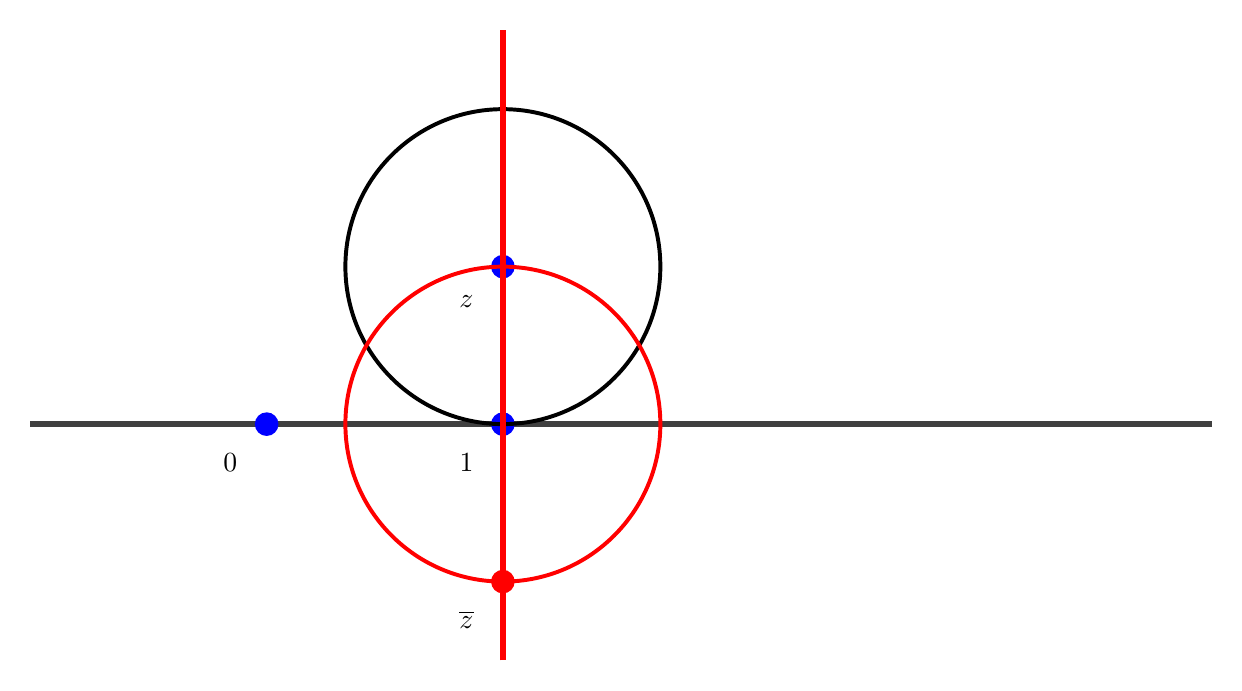
\begin{tikzpicture}
\draw[line width = 0.7mm, darkgray] (0,0) -- (15,0);
\fill[blue] (3,0) circle (0.15cm);
\fill[blue] (6,0) circle (0.15cm);
\fill[blue] (6,2) circle (0.15cm);
\node[below left=10pt] at (3,0) {$0$};
\node[below left=10pt] at (6,0) {$1$};
\node[below left=10pt] at (6,2) {$z$};
\draw[color=black, line width = 0.5mm] (6,2) circle [radius=2];
\draw[line width = 0.7mm, red] (6,-3) -- (6,5);
\draw[color=red, line width = 0.5mm] (6,0) circle [radius=2];
\fill[red] (6,-2) circle (0.15cm);
\node[below left=10pt] at (6,-2) {$\overline{z}$};
\end{tikzpicture}
\caption{- Example of case one of the proof of Lemma \ref{lemma:conjugate-in-Pn}}
\label{fig:case-1-conjugate}
\end{figure}
\FloatBarrier



\FloatBarrier
\begin{figure}[!hbt]
\centering
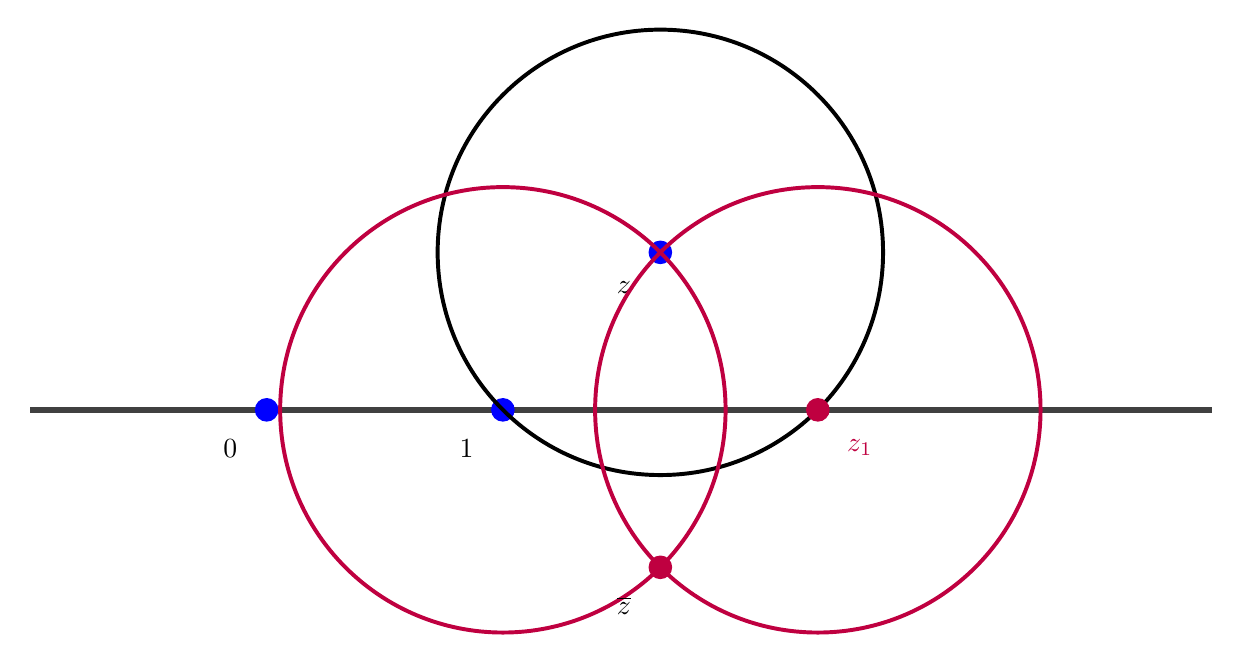
\begin{tikzpicture}
\draw[line width = 0.7mm, darkgray] (0,0) -- (15,0);
\fill[blue] (3,0) circle (0.15cm);
\fill[blue] (6,0) circle (0.15cm);
\node[below left=10pt] at (3,0) {$0$};
\node[below left=10pt] at (6,0) {$1$};
\fill[blue] (8,2) circle (0.15cm);
\node[below left=10pt] at (8,2) {$z$};
\draw[color=black, line width = 0.5mm] (8,2) circle [radius=2.828427];
\fill[purple] (10,0) circle (0.15cm);
\node[below right=10pt, color = purple] at (10,0) {$z_1$};
\draw[color=purple, line width = 0.5mm] (10,0) circle [radius=2.828427];
\draw[color=purple, line width = 0.5mm] (6,0) circle [radius=2.828427];
\fill[purple] (8,-2) circle (0.15cm);
\node[below left=10pt] at (8,-2) {$\overline{z}$};
\end{tikzpicture}
\caption{- Example of case two of the proof of Lemma \ref{lemma:conjugate-in-Pn}}
\label{fig:case-2-conjugate}
\end{figure}
\FloatBarrier

\begin{theorem}
    $\pi$ is not rational.
\end{theorem}

\begin{proof}

    \textcolor{red}{To Do:} Finish Proof
    Consider the following integral:

    $I_n = \int_{-1}^{1} (1-x^2)^ncos(\alpha x)dx$

    By integration by parts one time, we obtain that:

    $I_n = \frac{2n}{\alpha}\int_{-1}^{1}x\sin(\alpha x)(1-x^2)^{n-1}$
\end{proof}


\section{Diagrams}


\begin{figure}
	\centering
	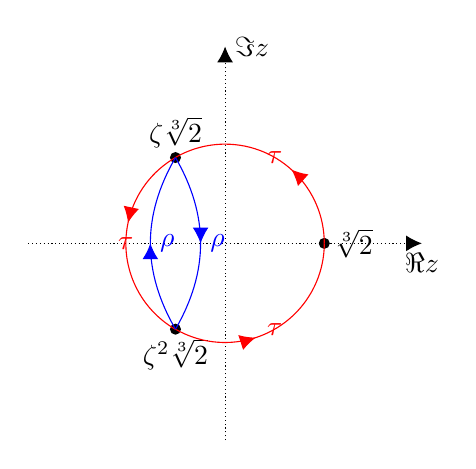
\begin{tikzpicture}
		\draw[->, densely dotted] (-2.5,0) -- (2.5,0) node[below] {$\Re z$};
		\draw[->, densely dotted] (0,-2.5) -- (0,2.5) node[right] {$\Im z$};
		%		\draw[densely dotted] (0, 0) circle (1); 
		%		\draw[densely dotted] (0, 0) circle (1.26); 
		
		\fill (1.26, 0) circle (2pt) node[right] {$\sqrt[3]{2}$};
		\fill (-0.63, 1.09) circle (2pt) node[above] {$\zeta \sqrt[3]{2}$};
		\fill (-0.63, -1.09) circle (2pt) node[below] {$\zeta^2 \sqrt[3]{2}$};
		%		\fill (1, 0) circle (1pt) node[left] {$1$};
		%		\fill (-0.5, -0.866) circle (2pt) node[above] {$\zeta^ 2$};
		%		\fill (-0.5, 0.866) circle (2pt) node[below] {$\zeta$};
		\draw[->-=0.4, red] (1.26, 0) arc   (0:120:1.26)  node[midway] {$\tau$};
		\draw[->-=0.4, red] (-0.63, 1.09) arc (120:240:1.26)  node[midway] {$\tau$};
		\draw[->-=0.4, red] (-0.63, -1.09) arc (240:360:1.26) node[midway] {$\tau$};
		\draw[->-=0.5, blue] (-0.63, -1.09) to [out=120,in=240] node[right] {$\rho$} (-0.63, 1.09); 
		\draw[->-=0.5, blue] (-0.63, 1.09) to [out=300,in=60] node[right] {$\rho$} (-0.63, -1.09); 
		
		
		
		%		\draw[very thin,color=gray] (-3,-3) grid (3,3);
	\end{tikzpicture}
	\caption{Actions of $\tau$ and $\rho$ on the roots of $f(t) = t^3 - 2$.}
	\label{fig:example-action}
\end{figure}

\begin{figure}
	\centering
	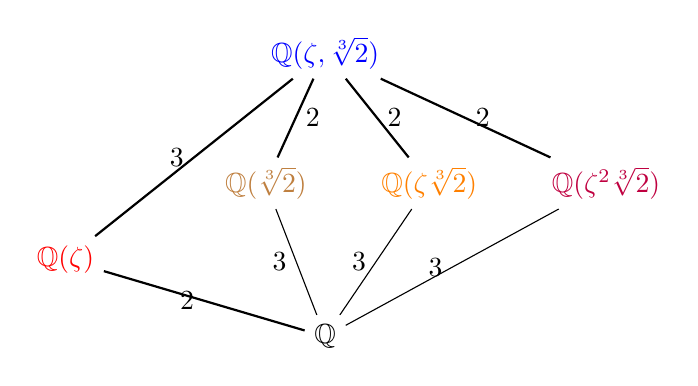
\begin{tikzpicture}
		
		\node(A1) 										{\textcolor{blue}{$\Q(\zeta, \sqrt[3]{2})$}};
		\node(B1) [below left=2cm and 2cm of A1]      	{\textcolor{red}{$\Q(\zeta)$}}; 
		\node(B2) [below left=1cm and -0.7cm of A1]     {\textcolor{brown}{$\Q(\sqrt[3]{2})$}}; 
		\node(B3) [right=0.7cm of B2]					{\textcolor{orange}{$\Q(\zeta \sqrt[3]{2} )$}}; 
		\node(B4) [right=0.7cm of B3]					{\textcolor{purple}{$\Q(\zeta^2 \sqrt[3]{2} )$}}; 
		\node(C1) [below=3cm of A1]						{$\Q$}; 
		
		\draw[thick](A1) -- node[left]{3} (B1); 
		\draw[thick](A1) -- node[right]{2} (B2); 
		\draw[thick](A1) -- node[right]{2} (B3); 
		\draw[thick](A1) -- node[right]{2} (B4); 
		
		\draw[thick](C1) -- node[left]{2} (B1); 
		\draw(C1) -- node[left]{3} (B2); 
		\draw(C1) -- node[left]{3} (B3); 
		\draw(C1) -- node[left]{3} (B4); 
		
	\end{tikzpicture}
	\caption{Lattice diagram for intermediate fields of $\Q(\zeta, \sqrt[3]{2})$, where $\zeta = e^{2\pi i / 3}$. Each line from a lower field $K$ to an upper field $L$ indicates a field extension $L/K$. The number on each line indicates the degree of $L/K$, i.e. $[L:K]$. A thick line indicates that $L/K$ is a normal (and Galois) extension. }
	\label{fig:example-intermidate-fields}
\end{figure}

\begin{figure} 
	\centering
	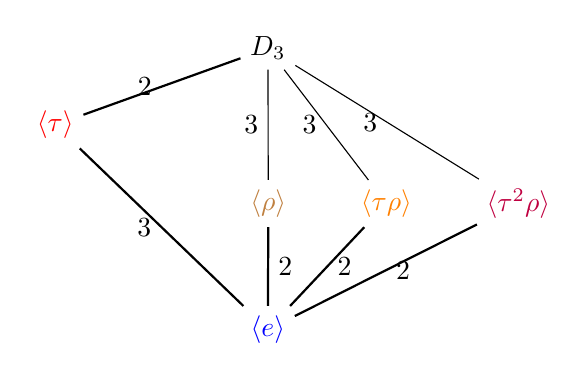
\begin{tikzpicture}
		\node(A1) 										{\textcolor{blue}{$\langle e \rangle$}};
		\node(B1) [above left=2cm and 2cm of A1]      	{\textcolor{red}{$\langle \tau \rangle$}}; 
		\node(B2) [above left=1cm and -0.7cm of A1]     {\textcolor{brown}{$\langle \rho \rangle$}}; 
		\node(B3) [right=0.7cm of B2]					{\textcolor{orange}{$\langle \tau \rho  \rangle$}}; 
		\node(B4) [right=0.7cm of B3]					{\textcolor{purple}{$\langle \tau ^ 2 \rho  \rangle$}}; 
		\node(C1) [above=3cm of A1]						{$D_3$}; 
		
		\draw[thick](A1) -- node[left]{3} (B1); 
		\draw[thick](A1) -- node[right]{2} (B2); 
		\draw[thick](A1) -- node[right]{2} (B3); 
		\draw[thick](A1) -- node[right]{2} (B4); 
		
		\draw[thick](C1) -- node[left]{2} (B1); 
		\draw(C1) -- node[left]{3} (B2); 
		\draw(C1) -- node[left]{3} (B3); 
		\draw(C1) -- node[left]{3} (B4); 
	\end{tikzpicture}
	\caption{Lattice diagram for subgroups of $D_3$. Each line from a lower group $H$ to an upper group $G$ indicates that $H$ is a subgroup of $G$. The number on each line indicates the index of $H$ in $G$, i.e. $[G:H]$. A thick line indicates that $H$ is a normal subgroup of $G$. }
	 \label{fig:example-subgroups}
\end{figure}


		




\newpage
% \bibliographystyle{abbrv}
\bibliography{bibliography}
\end{document}
